% License information <<<
%% Copyright 2019 Elsevier Ltd
%% 
%% This file is part of the 'CAS Bundle'.
%% --------------------------------------
%% 
%% It may be distributed under the conditions of the LaTeX Project Public
%% License, either version 1.2 of this license or (at your option) any
%% later version.  The latest version of this license is in
%%    http://www.latex-project.org/lppl.txt
%% and version 1.2 or later is part of all distributions of LaTeX
%% version 1999/12/01 or later.
%% 
%% The list of all files belonging to the 'CAS Bundle' is
%% given in the file `manifest.txt'.
%% 
%% Template article for cas-dc documentclass for 
%% double column output.

%\documentclass[a4paper,fleqn,longmktitle]{cas-dc}
% >>>
\documentclass[a4paper,fleqn]{cas-sc}

%\usepackage[authoryear,longnamesfirst]{natbib}
\usepackage[authoryear]{natbib}
\usepackage{amsmath}
\usepackage{gensymb}
\usepackage{subcaption}
\usepackage{siunitx}
\usepackage{setspace}
%\usepackage{lineno}
%\usepackage[numbers]{natbib}

%%%Author definitions
\def\tsc#1{\csdef{#1}{\textsc{\lowercase{#1}}\xspace}}
\tsc{WGM}
\tsc{QE}
\tsc{EP}
\tsc{PMS}
\tsc{BEC}
\tsc{DE}
%%%

%\linenumbers

\begin{document}
% Author particulars <<<
\let\WriteBookmarks\relax
\def\floatpagepagefraction{1}
\def\textpagefraction{.001}
\shorttitle{Energy Harvesting from an Angled Cruciform}
\shortauthors{A. Adzlan, M.S.M. Ali and S.A. Zaki}

\title [mode = title]{Vortex-induced Vibration of an Angled Cruciform for Energy Harvesting}                      
%\tnotemark[1,2]
%
%\tnotetext[1]{This document is the results of the research
%   project funded by the National Science Foundation.}
%
%\tnotetext[2]{The second title footnote which is a longer text matter
%   to fill through the whole text width and overflow into
%   another line in the footnotes area of the first page.}



\author[1,2]{Ahmad Adzlan}[orcid=0000-0003-0290-3185]
\cormark[1]
%\fnmark[1]
\ead{aafkhairi@graduate.utm.my}
%\ead[url]{www.cvr.cc, cvr@sayahna.org}

\credit{Conceptualisation, Methodology, Software, Validation, Formal analysis, Investigation, Data curation, Writing - Original draft preparation, Visualisation}

\address[1]{Malaysia-Japan International Institute of Technology, Universiti Teknologi Malaysia, 54200 Kuala Lumpur, Malaysia}

\author[1]{Mohamed Sukri Mat Ali}
%\fnmark[1]
\ead{sukri.kl@utm.my}
%\ead[URL]{www.sayahna.org}
\credit{Conceptualisation, Methodology, Resources, Writing - Review \& Editing, Supervision, Project administration, Funding acquisition}

\author[1]{Sheikh Ahmad Zaki}[orcid=0000-0001-6411-9965]
%\fnmark[1]
\ead{sheikh.kl@utm.my}
%\ead[URL]{www.sayahna.org}
\credit{Resources, Writing - Review \& Editing}

\address[2]{Faculty of Engineering, Universiti Malaysia Sarawak, 94300 Kota Samarahan, Sarawak, Malaysia}

\cortext[cor1]{Corresponding author}
%\cortext[cor2]{Principal corresponding author}
%\fntext[fn1]{This is the first author footnote. but is common to third
%  author as well.}
%\fntext[fn2]{Another author footnote, this is a very long footnote and
%  it should be a really long footnote. But this footnote is not yet
%  sufficiently long enough to make two lines of footnote text.}

%\nonumnote{This note has no numbers. In this work we demonstrate $a_b$
%  the formation Y\_1 of a new type of polariton on the interface
%  between a cuprous oxide slab and a polystyrene micro-sphere placed
%  on the slab.
%  }
% >>>
% Macros for commmon symbols <<<
\newcommand{\ypl}{y^{+}} %yPlus
\newcommand{\ured}{U^{*}} %reduced velocity
\newcommand{\yrms}{y^{*}_{\text{RMS}}} %root-mean-square of the normalised cylinder displacement
\newcommand{\ystr}{y^{*}} %the normalised cylinder displacement
\newcommand{\fstr}{f^{*}} %the normalised vibration frequency
\newcommand{\fn}{f_{n}} %system natural frequency
\newcommand{\fk}{f_{k}} %the coarsest grid in a grid independence study
\newcommand{\fvstr}{f^{*}_{v}} %normalise vortex shedding frequency
\newcommand{\fvk}{f_{v,\text{Karman}}} %Karman vortex shedding frequency
\newcommand{\fvkstr}{f^{*}_{v,\text{Karman}}} %normalised Karman vortex shedding frequency
\newcommand{\fcyl}{f_{\text{cyl.}}} %frequency of cylinder vibration
\newcommand{\fosc}{f_{\text{osc.}}} %frequency of cylinder oscillation
\newcommand{\fclstr}{f_{\text{Cl}}^{*}} %normalised frequency of lift coefficient
\newcommand{\flrms}{F_{\text{L,RMS}}} %root-mean-square of the lift force
\newcommand{\fl}{F_{\text{L}}} %the lift force
\newcommand{\clrms}{\text{Cl}_{\text{RMS}}} %root-mean-square of the lift coefficient
\newcommand{\cflyt}{C_{F_{L},y(t)}} %IMF component of lift that is most similar to the displacement signal in terms of temporal evolution of amplitude and frequency, differing only perhaps in phase OR the component of lift with the highest correlation to the displacement signal
\newcommand{\cflkrms}{C_{F_{L},\text{Karman},\text{RMS}}} %the Karman component of lift
\newcommand{\cflsrms}{C_{F_{L},\text{streamwise},\text{RMS}}} %the streamwise component of lift
\newcommand{\ccli}{C_{\text{Cl},i}} %the ith component of lift coefficient
\newcommand{\cclystr}{C_{\text{Cl},\ystr}} %the ith component of lift coefficient
\newcommand{\cflm}{C_{F_{L},\text{max}}} %IMF component of lift that has maximum RMS amplitude in the IMF set
\newcommand{\cyrms}{C_{y,\text{RMS}}} %the RMS of the component of lift that is most correlated with the cylinder displacement signal
\newcommand{\cclrms}{C_{\text{Cl},\text{RMS}}} %the RMS of the component of lift that is most correlated with the cylinder displacement signal (new symbol)
\newcommand{\cysys}{C_{\ystr,\ystr}} %the characteristic IMF representing the normalised cylinder displacement
\newcommand{\cclys}{C_{\text{Cl},\ystr}} %the characteristic IMF representing the lift coefficient
\newcommand{\afl}{\alpha_{F_{L}}} %ratio between two dominant IMF components of the lift

\newcommand{\angfi}{\SI{90}{\degree}} %90 deg. angle
\newcommand{\angfo}{\SI{67.5}{\degree}} %67.5 deg. angle
\newcommand{\angth}{\SI{45}{\degree}} %45 deg. angle
\newcommand{\angtw}{\SI{22.5}{\degree}} %22.5 deg. angle
\newcommand{\angon}{\SI{0}{\degree}} %0 deg. angle

\newcommand{\pfrms}{P_{\text{Fluid,RMS}}} %estimated root-mean-square of fluid power
\newcommand{\pmrms}{P_{\text{Mech.,RMS}}} %estimated root-mean-square of mechanical power
\newcommand{\etamech}{\eta_{\text{Mech.}}} %mechanical power efficiency
\newcommand{\re}{\text{Re}} %Reynolds number
\newcommand{\st}{\text{St}} %Strouhal number
\newcommand{\plag}{\theta_{y-\text{Cl}}} %Characteristic phase lag
\newcommand{\phim}{\phi_{\text{mean}}} %mean phase lag
\newcommand{\wcl}{W_{\text{cyl.}}} %mean work done by cylinder over one cycle of vibration
\newcommand{\tosc}{T_{\text{osc.}}} %mean period of cylinder oscillation
\newcommand{\meff}{m_{\text{eff.}}} %effective mass
\newcommand{\zetatot}{\zeta_{tot.}} %total damping of the system

%Macros that are shorthands in writing
\newcommand{\rms}{root-mean-square} %shorthand for root-mean-square

%Macros used in writing section on GCI study
\newcommand{\rp}{r^{p}} %refinement ratio, used in GCI study
\newcommand{\fre}{f_{\text{RE}}} %Richardson extrapolation of quantity of interest, used in GCI study

%The macros for freestream velocities
\newcommand{\uon}{\SI[per-mode=symbol]{0.1}{\metre\per\second}}
\newcommand{\utw}{\SI[per-mode=symbol]{0.2}{\metre\per\second}}
\newcommand{\uth}{\SI[per-mode=symbol]{0.3}{\metre\per\second}}
\newcommand{\ufo}{\SI[per-mode=symbol]{0.4}{\metre\per\second}}
\newcommand{\ufi}{\SI[per-mode=symbol]{0.5}{\metre\per\second}}
\newcommand{\usi}{\SI[per-mode=symbol]{0.6}{\metre\per\second}}
\newcommand{\use}{\SI[per-mode=symbol]{0.7}{\metre\per\second}}
\newcommand{\uei}{\SI[per-mode=symbol]{0.8}{\metre\per\second}}
\newcommand{\uni}{\SI[per-mode=symbol]{0.9}{\metre\per\second}}
\newcommand{\ute}{\SI[per-mode=symbol]{1.0}{\metre\per\second}}
\newcommand{\uel}{\SI[per-mode=symbol]{1.1}{\metre\per\second}}
\newcommand{\utv}{\SI[per-mode=symbol]{1.2}{\metre\per\second}}
\newcommand{\utt}{\SI[per-mode=symbol]{1.3}{\metre\per\second}}

\newcommand{\uron}{2.3}
\newcommand{\urtw}{4.5}
\newcommand{\urth}{6.8}
\newcommand{\urfo}{9.1}
\newcommand{\urfi}{11.4}
\newcommand{\ursi}{13.6}
\newcommand{\urse}{15.9}
\newcommand{\urei}{18.2}
\newcommand{\urni}{20.5}
\newcommand{\urte}{22.7}
\newcommand{\urel}{25.0}
\newcommand{\urtv}{27.3}
\newcommand{\urtt}{29.5}
% >>>
\begin{abstract}
  We numerically investigated the system response of a circular cylinder-strip plate cruciform oscillator at cruciform angles $\alpha = \angfi{}$, \angfo{}, \angth{}, \angtw{} and \angon{}. We examined the numerical model using the open source C++ library OpenFOAM within Reynolds number $1.1 \times 10^{3} \leq \text{Re} \leq 14.6 \times 10^{3}$. We identified three types of system response from the cruciforms examined: the pure cruciform response with power in the order of \SI{1}{\milli\watt} when reduced velocity $\ured \geq \urse$ and reaches maximum efficiency when $\ured = \urei$, the steep-angled cruciform response with sub-\si{\milli\watt} power output and maximum efficiency when $(\ured,\alpha\,[\si{\degree}]) = (\urtw,\angfo)$, and the shallow-angled cruciform response with power in the order of \SI{10}{\milli\watt} when $\ured \geq \urfo$ and maximum efficiency when $(\ured,\alpha\,[\si{\degree}]) = (\urfo,\angon)$. The high power output from the shallow-angled cruciforms are due to the shedding of three-dimensional Karman vortices seemingly resulting from coalescence of vortex structures shed from the upstream cylinder and downstream strip plate.
\end{abstract}
%%fakesection GraphicalAbstract
\begin{graphicalabstract}
  \centering
  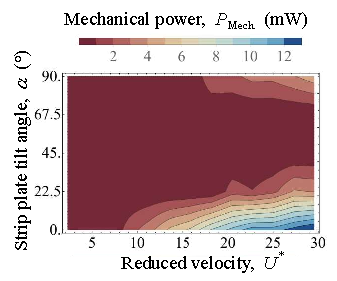
\includegraphics[width=0.4\textwidth]{figs/mechanicalPowerContours} \hspace{6mm} 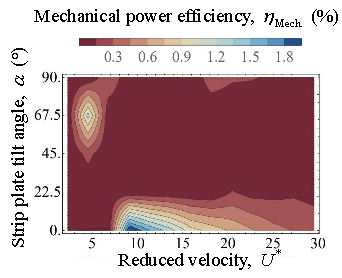
\includegraphics[width=0.4\textwidth]{figs/powerEfficiencyContours}

\end{graphicalabstract}

%%fakesection Highlights
\begin{highlights}
  \item Three main energy harvesting regimes were identified, based on the system response, mechanical power output and mechanical power efficiency of an angled cruciform oscillator.
  \item The pure cruciform (\angfi{}) produces maximum power in the order of \SI{1}{\milli\watt}, and maximum efficiency at reduced velocity $\ured = \urei$.
  \item The steep-angled cruciform (\angfo{} and \angth{}) produces maximum power in the order of \SI{0.001}{\milli\watt} to \SI{0.01}{\milli\watt}, and maximum efficiency at $(\ured,\alpha\,[\si{\degree}]) = (\urtw,\angfo)$.
  \item The shallow-angled cruciform (\angtw{} and \angon{}) produces maximum power in the order of \SI{10}{\milli\watt}, and maximum efficiency at $(\ured,\alpha\,[\si{\degree}]) = (\urfo,\angon)$.
  \item The region of high power output, resulting from shallow-angled cruciforms seems to be the driven by the shedding of three-dimensional Karman vortices with a very wide range of synchronisation.
\end{highlights}
\begin{keywords}
  Vortex-induced vibration \sep Vibration energy harvester \sep CFD simulation \sep Streamwise vorticity \sep Ensemble empirical mode decomposition (EEMD) \sep Hilbert transform
\end{keywords}


\maketitle

\doublespacing

\section{Introduction} \label{sec:intro}
The past two decades have witnessed an explosive growth in research concerning the field of energy harvesting from alternating lift mechanisms \citep{Ding2019,Xu2017,Sun2019b}. Contributors to this field focus mainly on the isolated circular cylinder oscillator, where previously unapplied ideas such as (1) operating the oscillator at high Reynolds number (Re) \citep{Bernitsas2008a,Bernitsas2009}, (2) imposing high mass-damping \citep{Lee2011a,Lee2011b,Sun2016} and (3) intentional oscillator symmetry breaking  \citep{Ding2015a,Ding2015b,Ding2017} lead to discoveries in the field that are directly related to improving the power output, operability range and efficiency of the energy harvester. A host of techniques were introduced into the field to facilitate new understanding and uncover perspectives previously unnoticed in the study of the isolated circular cylinder oscillator. For example, two-dimensional versions of the problem were investigated using computational fluid dynamics (CFD) \citep{Wu2011c,Zhang2018a}, implementation of virtual spring and damper in experimental works \citep{Garcia2018,Sun2018} and reliance on machine learning methods to explore the system response within a large parameter space \citep{Wu2018,Ren2019,Raissi2019,Hu2020} and also for active system control.

Almost concurrent with the developments in isolated circular cylinder research for energy harvesting is the accumulation of work on the cruciform oscillator. In its early days, the cruciform oscillator is nothing but two circular cylinders perpendicular to each other, overlapping at their midpoints \citep{Zdravkovich1981,Zdravkovich1983,Zdravkovich1985}. The elastically supported upstream cylinder is arranged parallel to the direction of freestream, while the downstream cylinder is fixed perpendicular to the upstream cylinder. Investigators observed the upstream cylinder acquiring significant vibrations in the scale of $O(10^{-1}D)$, as the reduced velocity of the flow $\ured$ exceeds 14. Here $D$ denotes the diameter of the upstream cylinder and the reduced velocity is defined in Eq. \ref{eq:reducedVelocity} as

\begin{equation}
  \ured = \frac{U_{\infty} \fn}{D},
  \label{eq:reducedVelocity}
\end{equation}

\noindent where $U_{\infty}$ and $\fn$ refers to the freestream velocity and the natural frequency of the system, respectively. More recent iterations of the system \citep{Koide2013,Koide2017} employs a thin, rectangular plate of width $w = D$ in place of the fixed downstream cylinder, and studies have shown that it retains most of the amplitude/frequency response of a two-circular cylinder cruciform.

However, at a gap $g$ of $0.16D$, or $G = g/D = 0.16$, researchers have found that the circular cylinder-strip plate oscillator managed to sustain its vibration over a very large range of $\ured$ \citep{Koide2013}. In relative terms, the vibration of this variant of the cruciform is sustained over a range of $\ured$ 15 times the width observed in an isolated, smooth circular cylinder oscillator of similar diameter \citep{Koide2009,Koide2013}. The reason behind this is the vortical structure driving the vibrations: vibration of the cruciform is driven by a pair of counter-rotating streamwise vortex shed a short distance from the cruciform juncture (refer Fig. \ref{fig:oscillatorSchematic}), while vibration of the isolated, smooth circular cylinder is driven by Karman vortices shed alternately from the top and bottom surface of the cylinder. The upside of this discovery is the fact that this wide synchronisation range is due to vortex shedding i.e., vortex-induced vibration (VIV) instead of galloping, as in \citet{Sun2019b}, \citet{Xu2019} and \citet{Ding2019}, as VIV-based energy harvesters of similar scale operate at higher efficiencies compared to galloping-based ones \citep{Sun2016,Ma2016}.

\begin{figure}
  \centering
  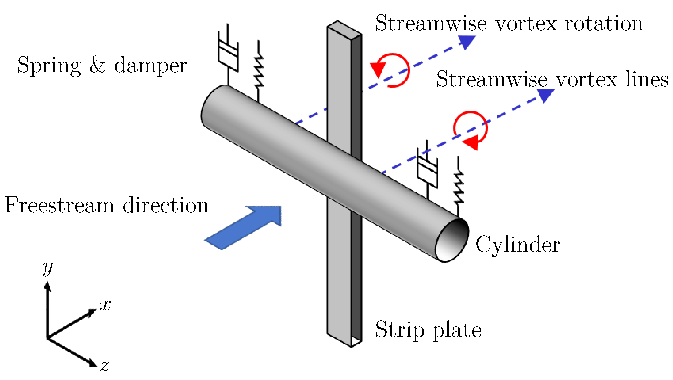
\includegraphics[width=0.5\textwidth]{figs/oscillatorSchematic}
  \caption{Schematic of the base configuration of the oscillator system used in this study, i.e. the pure cruciform. In this configuration, the axis of the cylinder and the strip plate are perpendicular to each other.}
  \label{fig:oscillatorSchematic}
\end{figure}

Despite this discovery, there is a paucity in efforts to test new streamwise vortex-based oscillators, especially those focusing on the passive control potential of the strip plate. The past three years saw a new direction taken in the study of cruciform systems, where investigators generalised the cruciform to an upstream circular cylinder and a downstream ring plate \citep{Hemsuwan2018a,Hemsuwan2018b,Hemsuwan2018c,Hemsuwan2018d}. The result of this setup is a steady lift energy harvester that is essentially a new type of turbine. We are not aware other attempts to generalise the cruciform structure for the purpose of improving its power output and efficiency as an alternating lift energy harvester.

Fully appreciating the potential role of the strip plate as a means to passively control the type of vortical structure, vibration response and power output/efficiency, we decide to address this gap in the following manner. We composed five different numerical models of the cruciform, all with an upstream circular cylinder and a downstream strip plate, but with differing cruciform angles $\alpha$ (\si{\degree}), starting from the pure cruciform (\angfi{}) down to the in-tandem arrangement (\angon{}) in \SI{22.5}{\degree} increments. Then, we performed transient three-dimensional Reynolds-averaged Navier-Stokes simulations with the models within $1.1 \times 10^{3} \leq \text{Re} \leq 14.6 \times 10^{3}$ ($\uron \leq \ured \leq \urtt$), and obtain the amplitude/frequency response, evolution of lift coefficient, and discuss the vortical structures central to the response. Finally, we mapped the mechanical power output and efficiency in the $\alpha$--$\ured$ parameter space to summarise the system response of the angled cruciform oscillator, and guide future prototype developments this system of energy harvesting.

\section{Methodology} \label{sec:method}
\subsection{Problem geometry} \label{ssec:probGeo}
This study bases itself on the work done by \citet{Maruai2017}, \citet{Maruai2018}, and \citet{Koide2013}. In these works, the investigators conducted both experimental and computational investigations of passive control of FSI of cylinders using a strip plate located at the cylinder downstream. Here, the term ``strip plate'' is used as a shorthand for the long, rectangular plate used to control the vibration of the cylinder -- since the plate resembles a strip due to its large aspect ratio. These studies demonstrated the feasibility of energy harvesting using the oscillator system described, in the Reynolds number range $3.6\times10^{3}<\text{Re}<12.5\times10^{3}$. Following this observation, we performed our numerical investigations within a similar \re{} range, albeit slightly widened, to check for variations in the cylinder response in as wide an \re{} range as possible, computational resources permitting.

Our oscillator system derives its geometry from the works of \citet{Nguyen2012}, \citet{Koide2013}, and \citet{Koide2017}. The basic layout of our oscillator system is the pure cruciform: an arrangement where the circular cylinder and the strip plate located downstream have their axes perpendicular to each other. We fixed the gap between the cylinder and the strip plate, $G$, to $0.16$. This value of $G$ was chosen because the cylinder response most suitable for energy harvesting is sustained over the largest range of reduced velocity $\ured$ when $G = 0.16$ \citep{Koide2013}.

\begin{figure}
  \centering
  \begin{subfigure}[h]{0.5\textwidth}
    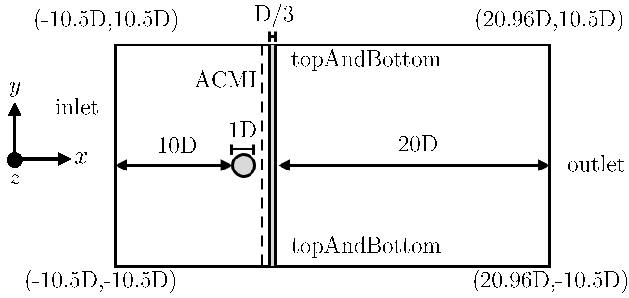
\includegraphics[width=\textwidth]{figs/problemGeometrySide}
    \caption{}
    \label{fig:probGeoSide}
  \end{subfigure}

  \begin{subfigure}[h]{0.5\textwidth}
    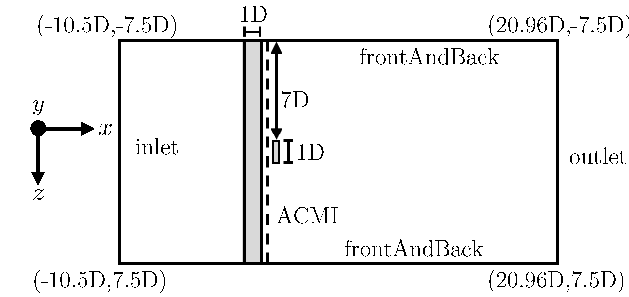
\includegraphics[width=\textwidth]{figs/problemGeometryTop}
    \caption{}
    \label{fig:probGeoTop}
  \end{subfigure}

  \caption{Figure \ref{fig:probGeoSide} shows the cross-sectional layout of the computational domain, along with key dimensions, when viewed from the side. Figure \ref{fig:probGeoTop} visualises the cross-section of the computational domain as viewed from the top. The arbitrarily coupled mesh interface (ACMI) used to connect the domain containing the cylinder with the domain containing the strip plate is placed halfway through the gap, i.e. $0.08D$ downstream the cylinder.} \label{fig:problemGeometry}
\end{figure}

Figure \ref{fig:probGeoSide} visualises our computational domain from its side. We chose these dimensions based on analogous works such as \cite{Maruai2017} and \cite{Maruai2018} which had produced results that agree well with experiments of their own and with \citet{Kawabata2013}. The streamwise coordinates of this domain extends from $-10.5D$ to $10.5D$, and the lateral coordinates from $-10.5D$ to $10.5D$. The coordinate origin $(0,0,0)$, is at the centre of the cylinder and the strip plate is $D/3$ thick.

In Fig. \ref{fig:probGeoTop}, the circular cylinder extends from $z/D=7.5$ to $z/D=-7.5$, giving the computational domain an overall spanwise length of $15D$. The computational domain of a similar study by \citet{Deng2007} has a length of $12D$, upon which the dimension of our domain is based upon. The extra $1.5D$ of spanwise length on either side of our domain is allocated to ensure the full expression of the three-dimensionality of flow structures that appear during the course of our numerical study.

\begin{figure}
  \centering
  \begin{subfigure}[h]{0.3\textwidth}
    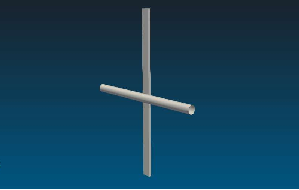
\includegraphics[width=\textwidth]{figs/cruciform90}
    \caption{Cruciform layout for \angfi{}}
    \label{fig:cruciform90}
  \end{subfigure}
  \hfill
  \begin{subfigure}[h]{0.3\textwidth}
    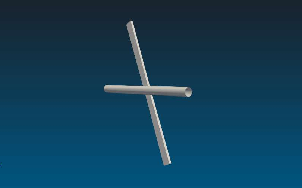
\includegraphics[width=\textwidth]{figs/cruciform675}
    \caption{Cruciform layout for \angfo{}}
    \label{fig:cruciform675}
  \end{subfigure}
  \hfill
  \begin{subfigure}[h]{0.3\textwidth}
    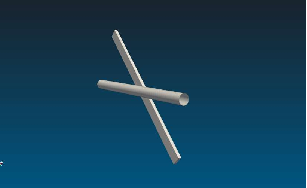
\includegraphics[width=\textwidth]{figs/cruciform45}
    \caption{Cruciform layout for \angth{}}
    \label{fig:cruciform45}
  \end{subfigure}

  \raggedright
  \begin{subfigure}[h]{0.3\textwidth}
    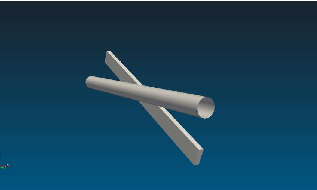
\includegraphics[width=\textwidth]{figs/cruciform225}
    \caption{Cruciform layout for \angtw{}}
    \label{fig:cruciform22.5}
  \end{subfigure}
  \hspace{6mm}
  \begin{subfigure}[h]{0.3\textwidth}
    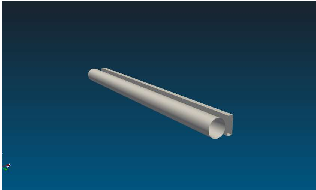
\includegraphics[width=\textwidth]{figs/cruciform00}
    \caption{Cruciform layout for \angon{}}
    \label{fig:cruciform00}
  \end{subfigure}

  \caption{Variation of cruciforms studied in this work. We vary the cruciform angle from the case of a pure cruciform (\angfi{}) to the case of cylinder - plate in tandem (\angon{}), in increments of \angtw{}.}\label{fig:cruciformLayouts}
\end{figure}

We then produce variants of the pure cruciform configuration by rotating the strip plate from \angfi{} to \angon{} in \angtw{} increments. In total, we constructed five different cruciforms shown in Fig. \ref{fig:cruciformLayouts}. The dimensions of the computational domain remain fixed for all cruciforms, including the gap between the cylinder and the strip plate.

\subsection{Numerical method} \label{ssec:numMeth}
Our numerical study utilises OpenFOAM, an open-source computational fluid dynamics (CFD) platform written in C++. With OpenFOAM, we solved the 3D unsteady Reynolds averaged Navier-Stokes (3D URANS) equations that are the following.

\begin{equation}
  \frac{\partial U_{i}}{\partial x_{i}}=0,
  \label{eq:continuity}
\end{equation}

\begin{equation}
  \frac{\partial U_{i}}{\partial t}+U_{j}\frac{\partial U_{i}}{\partial x_{j}} = -\frac{1}{p}\frac{P}{x_{i}}+\frac{\partial}{\partial x_{j}} \left( 2\nu S_{ij}-\overline{u'_{j}u'_{i}} \right).
  \label{eq:navier-stokes}
\end{equation}

The symbols $U$, $x$, $t$, $\rho$, $P$, $\nu$, $S$, and $u'$ denote the mean component of velocity, spatial component, time, density, pressure, kinematic viscosity, mean strain rate and the fluctuating component of velocity, respectively. Equation \ref{eq:sij} gives the mean strain rate $S_{ij}$.

\begin{equation}
  S_{ij} = \frac{1}{2} \left( \frac{\partial U_{i}}{\partial x_{j}} + \frac{\partial U_{j}}{\partial x_{i}} \right).
  \label{eq:sij}
\end{equation}

The turbulence model employed to approximate the Reynolds stress tensor is the Spalart-Allmaras turbulence model. Previous numerical studies on energy harvesting from FIM of circular cylinders have shown reasonable agreement with experiments in the literature through the use of this turbulence model, and thus becomes the basis for the implementation of the same turbulence model in our study \citep{Ding2015a,Ding2015b}. The Boussinesq approximation relates the Reynolds stress tensor $\tau_{ij} = \overline{u'_{j}u'{i}}$ to the mean velocity gradient, exemplified by Eq. \ref{eq:tauij}.

\begin{equation}
  \tau_{ij} = 2 \nu_{T}S_{ij},
  \label{eq:tauij}
\end{equation}

\noindent where $\nu_{T}$ represents the kinetic eddy viscosity. This kinetic eddy viscosity is ultimately expressed as a function whose arguments consist of the molecular viscosity $\nu$, and an intermediate variable $\tilde{\nu}$ that is the solution of Eq. \ref{eq:kineticEddyTransport}. Equation \ref{eq:kineticEddyTransport} incorporates empirically obtained constants to provide closure to the equations governing our numerical investigation. We list the empirical constants that make up Eq. \ref{eq:kineticEddyTransport} in Table \ref{tab:spalart-Allmaras}.

\begin{equation}
  \label{eq:kineticEddyTransport}
  \frac{\partial \tilde{\nu}}{\partial t} + U_{j} \frac{\partial \tilde{\nu}}{\partial x_{j}} = c_{b1}\tilde{S}\tilde{\nu} - c_{w1} f_{w} \left( \frac{\tilde{\nu}}{D} \right)^{2} + \frac{1}{\sigma} \left\{ \frac{\partial}{\partial x_{j}} \left[ \left( \nu + \tilde{\nu} \right) \frac{\partial \tilde{\nu}}{\partial x_{j}} \right] c_{b2} \frac{\partial \tilde{\nu}}{\partial x_{i}} \frac{\partial \tilde{\nu}}{\partial x_{i}} \right\}
\end{equation}

\begin{table}[width=0.6\textwidth,cols=2,pos=h]
  \caption{Empirical constants used in the Spalart-Allmaras turbulence model.} \label{tab:spalart-Allmaras}
  \begin{tabular*}{\tblwidth}{@{} LL@{} }
    \toprule
      Empirical constants & Value    \\
    \midrule
      $c_{b1}$            & $0.01$   \\
      $c_{b2}$            & $0.09$   \\
      $c_{\nu1}$          & $0.01$   \\
      $\kappa$            & $0.1$    \\
      $\sigma$            & $0.162$  \\
      $c_{\omega3}$       & $0.178$  \\
    \bottomrule
  \end{tabular*}
\end{table}

\noindent We refer the interested reader to the original paper by \citet{Spalart1992} and more recent applications of the turbulence model in \citet{Ding2019} and \citet{Sun2019b}. With the turbulence model properly defined, we are finally able to solve Eqs. \ref{eq:continuity} and \ref{eq:navier-stokes} using the SIMPLE-stabilised PISO algorithm native to OpenFOAM, known as the PIMPLE algorithm. 

\subsection{Dynamic mesh motion} \label{ssec:dynMesh}

Cylinder motion in the computational domain due to FIV introduces distortion to the mesh immediately surrounding the cylinder. The simplest way to keep the mesh distortion in check, thus keeping mesh quality within an acceptable level, is by diffusing the amount of warping to the surrounding space. In practice, the surrounding space is the rest of the mesh nodes, and Eq. \ref{eq:laplace} governs the diffusion.

\begin{equation}
  \nabla \cdot \left( \gamma \nabla u \right) = 0.
  \label{eq:laplace}
\end{equation}

In Eq. \ref{eq:laplace}, $u$ and $\gamma$ represents the mesh deformation velocity and displacement diffusion, respectively. In this work, we set the displacement to be diffused according to the inverse quadratic rule $\gamma = 1/l^{2}$. Here, $l$ denotes the distance from the cell centre to the nearest cylinder edge. Then, we solve Eq. \ref{eq:laplace} using the GAMG algorithm and the Gauss-Seidel smoother. Solution of Eq. \ref{eq:laplace} returns an updated value of $u$, and this updated value of $u$ is used to update the position of the mesh nodes according to Eq. \ref{eq:meshNodeUpdate}. The PIMPLE solver resumes the solution of the 3D URANS equations after we update the mesh node positions.

\begin{equation}
  x_{\text{new}} = x_{\text{old}} + u \Delta t
  \label{eq:meshNodeUpdate}
\end{equation}

For most numerical studies of FSI, the mesh warp diffusion method governed by Eq. \ref{eq:laplace} serves as an adequate workaround to conserve mesh quality. However, this requires ample number of ambient mesh nodes acting as the receiving end of the diffusion algorithm. In our case, the small gap between the cylinder and strip plate ($G = 0.16$) pose a serious limitation to our ability to diffuse the amount of warp introduces by the displacement of the cylinder, since a small space means that we can only allocate a proportionate number of mesh nodes in said gap. Sole reliance on the warp diffusion algorithm will hamper our effort to preserve mesh quality as a high concentration of warp remains within the gap. To overcome this problem, we implement the arbitrarily coupled mesh interface (ACMI) halfway through the gap (see Fig. \ref{fig:problemGeometry}). This technique allows adjacent cells to slide over each other precisely at the $x = 0.13$ plane, ridding us of the requirement for mesh warp diffusion. In the literature, ACMI is also known as the generalised grid interface, or GGI \citep{Zhang2018,Sun2019b}.

\subsection{Open flow channel experiment} \label{ssec:openFlowExp}

As part of the validation process for our numerical setup, we constructed a closed loop open flow channel, with a test section \SI{100}{\milli\metre} wide, \SI{200}{\milli\metre} high and \SI{1500}{\milli\metre} long. The design of this open flow channel is heavily inspired by the water tunnel of \citet{Nguyen2012} and \citet{Koide2013}. Considering the application of this research in the far future is in open flows such as natural drainage systems or the ocean - and not within pipes - prompts us to make this distinction.

We benchmark the open flow channel by setting up a pure cruciform oscillator (\angfi{}) experiment, whose data from similar studies are readily available in published works. Following this, we dimensioned the rig to follow the parameters used in \citet{Koide2013}. A summary of our parameters and those used in \citet{Koide2013} are provided in Table \ref{tab:expParameter}. We tune the parameters governing the amplitude/frequency response of the oscillator using simple length-based mechanism as follows (see Fig. \ref{fig:rigSketch}). To tune the spring coefficient $k$, we simply adjust the active length of the twin spring plate. In practice, we obtained the calibration curve of the twin spring plate by performing a weight - displacement measurement \citep{Sun2016} at several active lengths of the plate. Once the spring coefficient versus spring plate active length calibration curve is obtained, we can just adjust the length of the spring plate to achieve the desired value of $k$.

\begin{figure}
  \centering
  \begin{subfigure}[h]{0.5\textwidth}
    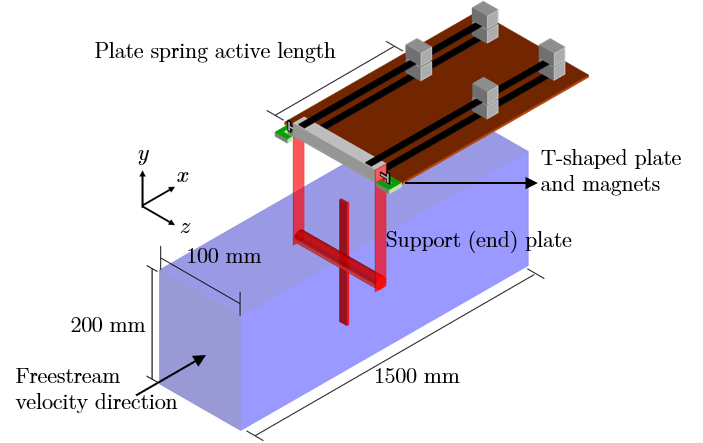
\includegraphics[width=\textwidth]{figs/rigSketch}
    \caption{}
    \label{fig:rigSketch}
  \end{subfigure}

  \begin{subfigure}[h]{0.35\textwidth}
    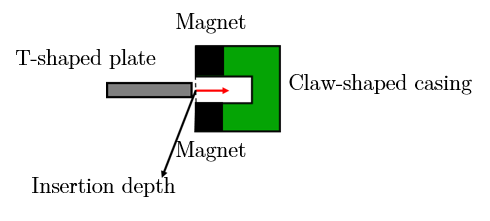
\includegraphics[width=\textwidth]{figs/damperSketch}
    \caption{}
    \label{fig:damperSketch}
  \end{subfigure}

  \caption{Our experimental system used to validate our numerical study. Figure \ref{fig:rigSketch} presents a 3D schematic of the open channel test section with a pure cruciform oscillator setup, while Fig. \ref{fig:damperSketch} shows a magnified schematic of the damping system.} \label{fig:experimentalSetup}
\end{figure}

Tuning the total damping of the system and consequently the multiple expressions of damping such as the logarithmic damping $\delta$, Scruton number Sc, or the damping coefficient is done by attaching, as shown in Fig. \ref{fig:rigSketch}, a T-shaped plate made from aluminium into a claw-shaped casing that houses neodymium magnets at its ends. As presented in Fig. \ref{fig:damperSketch}, the method we use to control the strength of the magnetic field exposed to the T-shaped plate is by fixing the insertion depth of the T-shaped plate into the casing. The magnetic field serves to dissipate the kinetic energy of the T-shaped plate that moves with the cylinder during FIM, providing system damping.

\begin{table}[width=0.9\linewidth,cols=3,pos=h]
  \caption{Summary of experimental parameters in contrast to those used in the experimental work of \citet{Koide2013}.} \label{tab:expParameter}
\begin{tabular*}{\tblwidth}{@{} LLL@{} }
\toprule
                                           & Current study & \citet{Koide2013}\\
\midrule
Cylinder diameter, $D$ (m)                 & $0.01$        & $0.01$           \\
Cylinder length, $l_{\text{cylinder}}$ (m) & $0.09$        & $0.098$          \\
Strip-plate width (m)                      & $0.01$        & $0.01$           \\
Strip-plate length (m)                     & $0.1$         & $0.1$            \\
Effective mass, $m_{\text{eff.}}$ (kg)     & $0.162$       & $0.174$          \\
Logarithmic damping, $\delta$              & $0.178$       & $0.24$           \\
Scruton number, Sc                         & $9.94$        & $7.74$           \\
System natural frequency, $f_{n}$ (Hz)     & $4.42$        & $4.4$ to $4.79$  \\
\bottomrule
\end{tabular*}
\end{table}

A voltage controller regulates the power driving the $3.728$ kW (5 hp) centrifugal pump. To set the freestream velocity in the open flow channel, we placed an acoustic Doppler velocimeter (ADV) sampling at in an empty test section, filled with plain tap water to a height of \SI{100}{\milli\metre}, on the centreline of the channel, as pictured in Fig. \ref{fig:channelSchematic}. The height of \SI{100}{\milli\metre} is also the water level we conduct our experiments in. We keep the water level at this height of \SI{100}{\milli\metre} during all data collections to achieve a flow ambience analogous to our benchmark study of \citet{Koide2013}, facilitating comparison between the two. Then, we sampled the velocity of the flow at different input voltages by the voltage controller, the final product being an input voltage $V_{\text{in}}$ (V) versus centreline velocity $U_{\text{cent.}}$ calibration curve. This calibration curve allows us to set the freestream velocity of the open flow channel by specifying the input voltage to the pump. The finished product gave an operability range between \uth{} and \uel{}, which translates to $\urth \leq \ured \leq \urel$ for an circular cylinder of diameter \SI{10}{\milli\metre}. The turbulence level ranges between $5\%$ to $8\%$ when the freestream velocity $U_{\infty} \geq \uei$.

\begin{figure}
  \centering
  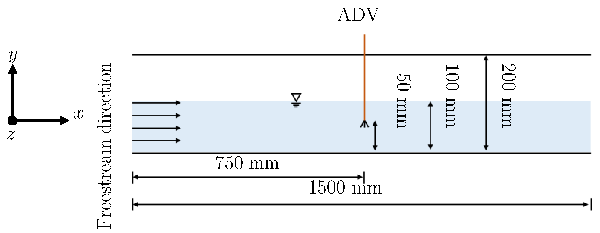
\includegraphics[width=0.6\textwidth]{figs/channelSchematic}
  \caption{The side view of our test section. For a more valid benchmarking of our open channel flow with a similar system in \citet{Koide2013}, we keep the water level to \SI{100}{\milli\metre}.}
  \label{fig:channelSchematic}
\end{figure}

We measured the cylinder displacement $y$ as a function of time by placing a visual marker on the support plate of the cylinder (see Fig. \ref{fig:rigSketch}) and capturing the motion of the marker using a video camera positioned perpendicular to the support plate. The motion of the marker is then analysed using \textit{Tracker}: a motion analysis tool built on the Open Source Physics Java framework (for recent implementation examples, see \citet{Wen2020}  or \citet{Krishnendu2020}).

For the benchmarking, we chose the reduced velocity $\ured = \urte$, as the cylinder at that $\ured$ produces a large and stable displacement that simplifies on our part, the measurement and comparison process between our experimental system and \citet{Koide2013}. A sample of the normalised displacement -- $\ystr = y/D$ -- measured as a function of time is illustrated in Fig. \ref{fig:sampTimeHist}. This time series allows us to also compute the normalised cylinder vibration frequency, $\fstr = \fcyl/\fn$ ($\fcyl$ being the vibration frequency of the cylinder). The $\ystr$ data presented in Fig. \ref{fig:sampTimeHist} returns $\ystr = 0.33 \pm 0.03$ and $\fstr 1.03 \pm 0.04$, after computing the uncertainty from multiple experimental runs. In their work, \citet{Koide2013} obtained $\ystr = 0.32$ and $\fstr = 1.09$ at a similar $\ured$ - values that are well within the measurement uncertainty of our experiment. This provides a basis for our reliance on results obtained from the experimental system later in the study.

\begin{figure}
  \centering
  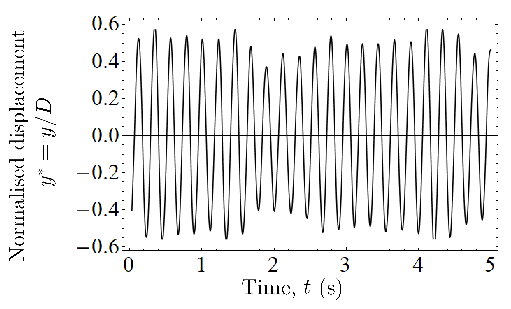
\includegraphics[width=0.41\textwidth]{figs/figure5}
  \caption{The normalised cylinder displacement measured as a function of time at $\ured = \urte$. The experiment was repeated several times to estimate the uncertainty of the measured quantities $\ystr$ and $\fstr$.}
  \label{fig:sampTimeHist}
\end{figure}

\section{Numerical setup validation} \label{sec:numSetup}
\subsection{Richardson extrapolation and the grid convergence index (GCI)} \label{ssec:richExtrap}
In this work, we establish the grid independency of the solution using the Richardson extrapolation and the grid convergence index (GCI) \citep{Richardson1927,Stern2001}. The Richardson extrapolation and GCI provides us with a procedure to quantitatively measure on the degree of convergence for the quantities of interest in a numerical study. This method also forces us to pay attention to the trend of convergence of the quantities of interest, requiring a monotonic convergence before proceeding to data collection \citep{Stern2001,MatAli2011,Ali2012,Maruai2018}.

Let $f_{1},f_{2},f_{3},\dots,\fk$ be the quantity of interest obtained from several grid resolutions. We assign a larger subscript for a coarser grid, thus ascribing $f_{1}$ to the finest and $\fk$ to the coarsest grid. Let the difference between successive solutions be $\epsilon_{2,1},\epsilon_{3,2},\epsilon_{4,3},\dots,\epsilon_{n,n-1}$, where $\epsilon_{2,1} = f_{2} - f_{1}$, $\epsilon_{3,2} = f_{3} - f_{2}$ and so on. Then, the GCI is defined as

\begin{equation}
  \text{GCI}_{i+1,i} = F_{s} \frac{\left |\epsilon_{i+1,i} \right |}{f_{i} \left ( r^{p} - 1 \right )} \times 100\%,
  \label{eq:gci}
\end{equation}

\noindent where $F_{s}$, $f_{i}$ and $r^{p}$ denotes the safety factor $\left ( = 1.25 \right )$, quantity of interest and the refinement ratio, $r$, between successive grids raised to the order of accuracy of the series of solution, $p$. We refer the reader to \citet{Stern2001,Langley2018} for a more detailed discussion on $r^{p}$.

We can estimate the limit of the solution as the spacing between grid points approache zero via the $\text{p}^{\text{th}}$ method. In essence, we compute the generalised Richardson extrapolation of the quantity of interest as follows.

\begin{equation}
  \fre = f_{1} + \frac{f_{1} - f_{2}}{\rp - 1},
  \label{eq:richardsonExtrapolation}
\end{equation}

\noindent where $\fre$ is the Richardson extrapolation of the quantity of interest. Using $\fre$ to estimate the limit of the monotonically convergent series of $f_{i}$, we can determine the percentage difference of our solution on our finest grid from this limit as

\begin{equation}
  E_{i} = \frac{f_{i} - \fre}{\fre} \times 100\%.
  \label{eq:percentageDifference}
\end{equation}

Table \ref{tab:gridIndependency} summarises the result of our grid independency study for the SVIV reduced velocity of $\ured = 22.7$. The flow global quantities we check for convergence are the vibration amplitude, vibration frequency and lift coefficient of the cylinder. To simplify our grid independency study, we chose the pure cruciform configuration (the \angfi{} cruciform) as the representative, and collected data at $\ured = \urte$ on three sets of grid numbered $1$ for the finest, $2$ for the medium and $3$ for the coarsest, shown in Fig. \ref{fig:convergenceStudy}. With $v_{i}$ as the volume of the $i^{\text{th}}$ cell in the grid, and $N$ the total number of cells in our domain, the average cell size becomes

\begin{figure}
  \centering
  \begin{subfigure}[h]{0.3\textwidth}
    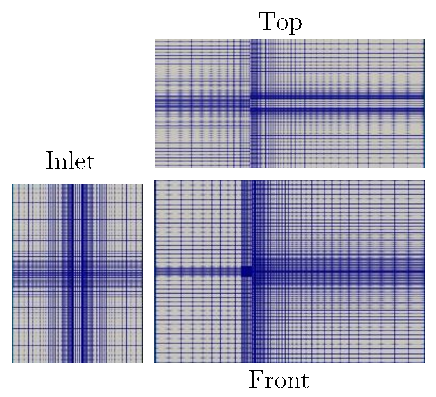
\includegraphics[width=\textwidth]{figs/figure6a}
    \caption{Coarse}
    \label{fig:coarseMesh}
  \end{subfigure}
  \hfill
  \begin{subfigure}[h]{0.3\textwidth}
    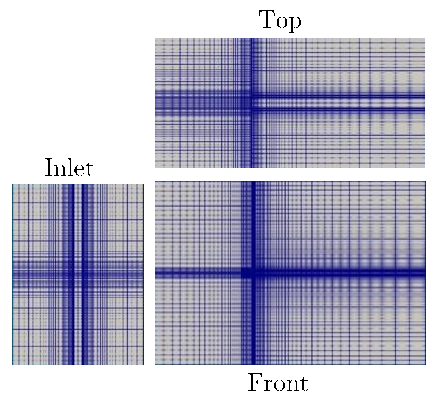
\includegraphics[width=\textwidth]{figs/figure6b}
    \caption{Medium}
    \label{fig:mediumMesh}
  \end{subfigure}
  \hfill
  \begin{subfigure}[h]{0.3\textwidth}
    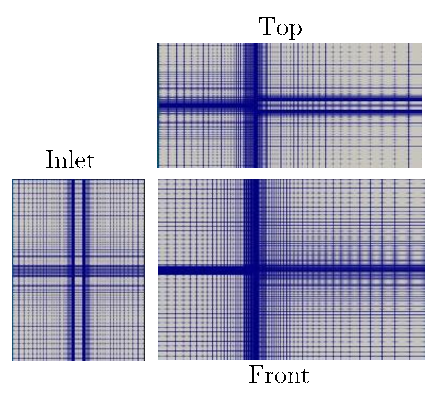
\includegraphics[width=\textwidth]{figs/figure6c}
    \caption{Fine}
    \label{fig:fineMesh}
  \end{subfigure}

  \caption{Three meshes used in the grid convergence study. Figures \ref{fig:coarseMesh}, \ref{fig:mediumMesh} and \ref{fig:fineMesh} show the coarse, medium and fine meshes viewed perpendicular to three main viewing positions: from the inlet, the top and the front, which is looking directly at the cylinder end.} \label{fig:convergenceStudy}
\end{figure}

\begin{equation}
  h = \frac{1}{N} \left [ \sum_{i=1}^{N} v_{i} \right ]^{1/3},
  \label{eq:averageCellSize}
\end{equation}

\noindent and the normalised average cell size is hence 


\begin{equation}
  h/D = \frac{1}{ND} \left [ \sum_{i=1}^{N} v_{i} \right ]^{1/3}.
  \label{eq:normAveCellSize}
\end{equation}

\noindent Both $\yrms$ and $\clrms$ (see Figs. \ref{fig:gciYrms} and \ref{fig:gciClrms}) have initial values smaller than their Richardson extrapolations, $\fre$, before approaching $\fre$, with decreasing $h$. The vibration frequency, on the other hand, starts at a value larger than its $\fre$ before approaching $\fre$, as one can see in Fig. \ref{fig:gciFstr}.

The most significant drop in GCI is experienced by $\clrms$, with increasing refinement of the grid. Refinement from the coarse to medium grid returns a GCI of $30.92\%$, using a refinement ratio of $1.376$. We compute the refinement ratio by dividing the number of cells in one grid with the grid one stage refined. Generalising this to $i$ number of grids returns

\begin{equation}
  r_{i+1,i} = \frac{S_{\text{grid},i+1}}{S_{\text{grid},i}},
  \label{eq:refinementRatio}
\end{equation}

\noindent where $S_{\text{grid},i}$ denotes the total number of cells in the $i^{\text{th}}$ grid. The GCI of $\clrms$ decreases further to $1.63\%$ with further refinement of the grid. On the other hand, GCI for $\fstr$, shrinks to about one-sixth of its former value.

\begin{table}[width=0.9\linewidth,cols=4,pos=h]
  \caption{Summary of grid independency study.} \label{tab:gridIndependency}
\begin{tabular*}{\tblwidth}{@{} LLLL@{} }
\toprule
Parameter/ metric                                                       & $\clrms$       & $\yrms = \ystr/D$ & $\fstr = \fcyl / \fn$ \\
\midrule
$\fre$                                                                  & $0.262$        & $0.369$           & $0.969$               \\
$f_{1}$                                                                 & $0.2598$       & $0.3687$          & $0.9695$              \\
$f_{2}$                                                                 & $0.2430$       & $0.3588$          & $0.9740$              \\
$f_{3}$                                                                 & $0.0805$       & $0.2374$          & $1.0220$              \\
$\left | \epsilon_{2,1} \right |$                                       & $0.02$         & $0.01$            & $0.004$               \\
$\left | \epsilon_{2,1} \right |$                                       & $0.16$         & $0.12$            & $0.48$                \\
$R = \left | \epsilon_{2,1} \right | / \left | \epsilon_{2,1} \right |$ & $0.10$         & $0.08$            & $0.094$               \\
$\text{GCI}_{3,2}$ (\%)                                                 & $30.92$        & $6.00$            & $0.64$                \\  
$\text{GCI}_{3,2}$ (\%)                                                 & $1.63$         & $0.52$            & $0.10$                \\
\bottomrule
\end{tabular*}
\end{table}

Inspecting Figs. \ref{fig:gciYrms}, \ref{fig:gciFstr} and \ref{fig:gciClrms}, we find the quantities of interest to be very close to its Richardson extrapolation at the fine grid (grid 1) for all $\clrms$, $\yrms$ and $\fstr$. We take this as an indication of sufficient spatial discretisation. At this point, we find the trade-off between a solution even closer to the Richardson extrapolation and the increased computational effort no longer appealing, compounded by our observation that values of $\yrms$ and $\fstr$ at the fine grid already fall within experimental uncertainty as evidenced by our measurement in \S \ref{ssec:openFlowExp} and the work by \citet{Koide2013}. We use the fine grid in all simulations of the pure cruciform case, and implemented a similar mesh resolution to all cruciform variants studied in this work.

\begin{figure}
  \centering
  \begin{subfigure}[h]{0.38\textwidth}
    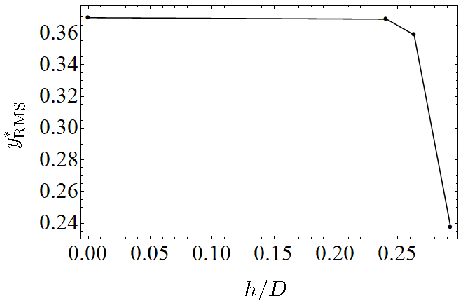
\includegraphics[width=\textwidth]{figs/gciYrms-1}
    \caption{}
    \label{fig:gciYrms-1}
  \end{subfigure}
  \hspace{6mm}
  \begin{subfigure}[h]{0.38\textwidth}
    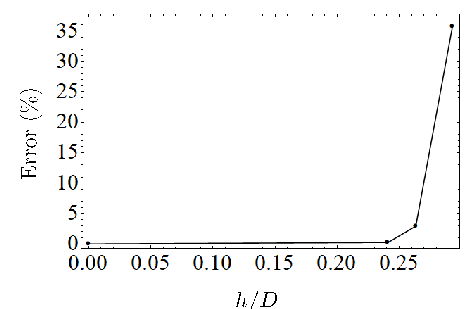
\includegraphics[width=\textwidth]{figs/gciYrms-2}
    \caption{}
    \label{fig:gciYrms-2}
  \end{subfigure}

  \caption{The convergence diagram for $\yrms$. Figure \ref{fig:gciYrms-1} shows how $\yrms$ converges close to the Richardson extrapolation value while Fig. \ref{fig:gciYrms-2} shows how the error (difference between the value obtained from a particular mesh and the Richardson extrapolation) decreases with decreasing grid spacing.} \label{fig:gciYrms}
\end{figure}

\begin{figure}
  \centering
  \begin{subfigure}[h]{0.39\textwidth}
    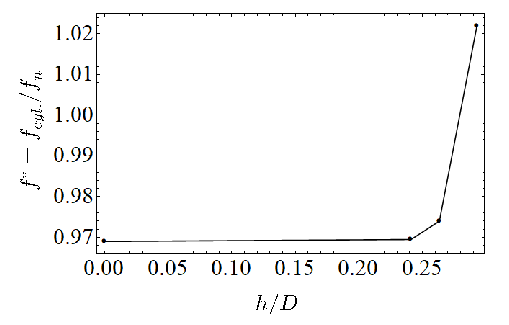
\includegraphics[width=\textwidth]{figs/gciFstr-1}
    \caption{}
    \label{fig:gciFstr-1}
  \end{subfigure}
  \hspace{6mm}
  \begin{subfigure}[h]{0.39\textwidth}
    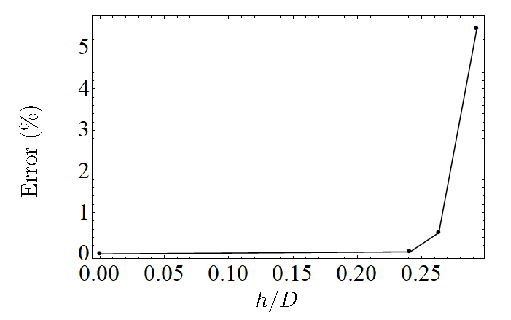
\includegraphics[width=\textwidth]{figs/gciFstr-2}
    \caption{}
    \label{fig:gciFstr-2}
  \end{subfigure}
  \caption{The convergence diagram for $\fstr$. Figure \ref{fig:gciFstr-1} shows how $\fstr$ converges close to the Richardson extrapolation value while Fig. \ref{fig:gciFstr-2} shows how the error (difference between the value obtained from a particular mesh and the Richardson extrapolation) decreases with decreasing grid spacing.} \label{fig:gciFstr}
\end{figure}

\begin{figure}
  \centering
  \begin{subfigure}[h]{0.39\textwidth}
    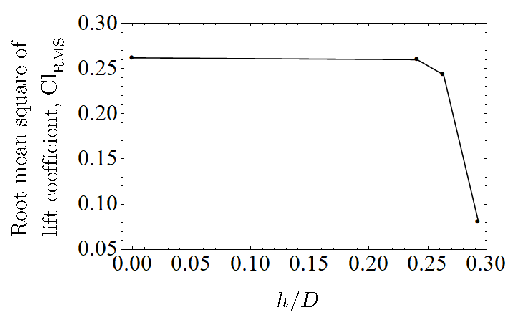
\includegraphics[width=\textwidth]{figs/gciClrms-1}
    \caption{}
    \label{fig:gciClrms-1}
  \end{subfigure}
  \hspace{6mm}
  \begin{subfigure}[h]{0.39\textwidth}
    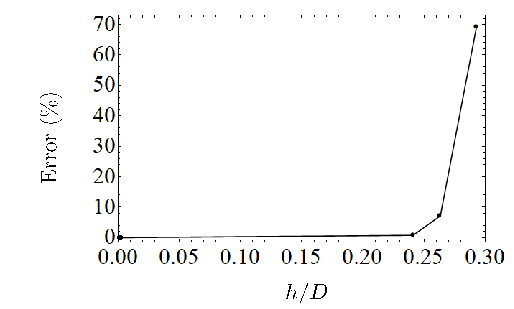
\includegraphics[width=\textwidth]{figs/gciClrms-2}
    \caption{}
    \label{fig:gciClrms-2}
  \end{subfigure}
  \caption{The convergence diagram for $\clrms$. Figure \ref{fig:gciClrms-1} shows how $\clrms$ converges close to the Richardson extrapolation value while Fig. \ref{fig:gciClrms-2} shows how the error (difference between the value obtained from a particular mesh and the Richardson extrapolation) decreases with decreasing grid spacing.} \label{fig:gciClrms}
\end{figure}

\section{Streamwise vortex-driven vibration}\label{sec:svivRegime}

\subsection{The amplitude and frequency response}\label{ssec:svivRegimeAmpFreqResp}

The pure cruciform case, i.e. \angfi{}, demonstrated a normalised \rms{} amplitude of cylinder displacement, $\yrms$ that starts quite expectedly with a low amplitude at reduced velocities $\uron$ and $\urtw$ , before reaching a value close to $\yrms = 0.1$ at $\ured = \urth$, as presented in Fig. \ref{fig:yStrRMS1}. Following the local maximum at $\ured = \urth$, $\yrms$ tapers off to less than $\yrms = 0.05$ between $\urfo \leq \yrms \leq \ursi$. This whole $\yrms$ trend of hitting a local maximum before tapering off bears a striking resemblance to the amplitude response of an isolated circular cylinder in KVIV at mass ratios of order $O(10^{1})$ \citep{Feng1963,Khalak1999}. This resemblance can be seen as an indication that the vibration of a pure cruciform between $\ured \leq \urse$ is driven primarily through the shedding cycle of Karman vortices.

\begin{figure}
  \centering
  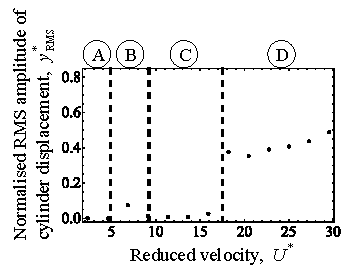
\includegraphics[width=0.38\textwidth]{figs/yStrRMS1}
  \caption{Evolution of the normalised \rms{} amplitude of cylinder displacement $\yrms$, with respect to reduced velocity $\ured$, in the streamwise vortex-driven vibration regime.} \label{fig:yStrRMS1}
\end{figure}

Then at $\ured = \urse$, $\yrms$ experiences a very weak increase followed by a sudden jump close to $0.4$ at $\ured = \urei$. This is followed by a slight decline at $\ured = \urni$ and return to the previous level of $\yrms$ at $\ured = \urte$. Past $\ured = \urte$, we observe that $\yrms$ maintains a linear trend in its variation with respect to $\ured$. As $\ured = \urei$ is well within the lower branch for a system in KVIV, it is quite unlikely for the vibration within $\urei \leq \ured \leq \urtt$ to be the governed by the shedding of Karman vortices, leading previous investigators to attribute the vibration to the periodic shedding of streamwise vortical structures dominating the spatial region close to the cruciform juncture \citep{Shirakashi1989,Hemsuwan2018b,Hemsuwan2018d}. Hence, we name this range of $\ured$ the streamwise vortex-induced vibration regime.

\begin{figure}
  \centering
  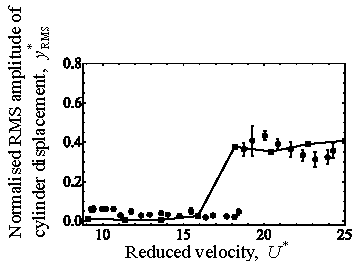
\includegraphics[width=0.4\textwidth]{figs/expCompareAmp}
  \caption{Comparison between the evolution of $\yrms$ with respect to $\ured$of a pure cruciform system from our numerical and experimental work. The filled square represents the numerical, while the filled circle represents the experimental results.}
  \label{fig:expCompareAmp}
\end{figure}

The experimental system consisting of the closed loop open flow channel and the pure cruciform oscillator rig in \S\ref{ssec:openFlowExp} is constructed not only for the purpose of validating the results of our pure cruciform numerical investigation, but also to corroborate in general, the sum total of our numerical setup. Admittedly, the best undertaking would be to perform equivalent experiment for each of the \angfi{}, \angfo{}, \angth{}, \angtw{} and \angon{} configurations, but the scale of such an exercise and subsequent discussion of the results in our opinion, deserves its own treatment separate from the current study. The degree of agreement between the results of our numerical and experimental investigation of the pure cruciform establishes the validity of our numerical setup, which we assume to extend to the rest of the cruciforms. We think that this assumption is somewhat founded because all cruciforms are simulated under similar boundary conditions, mesh resolution and solver algorithm.

Our experiments collect time series data of cylinder displacement $y$, from which the normalised \rms{} amplitude $\yrms$ is computed. Figure \ref{fig:expCompareAmp} compares both our numerical and experimental results of $\yrms$. We observe that both results agree in terms of magnitude and trend of the amplitude response. However, the jump to SVIV occurs at a higher $\ured \approx 19$, translating to a delay of about 3 units of $\ured$. Our numerical and experimental results are also able to capture the slight dip in $\yrms$ following the jump to SVIV, but the occurrence in our experiment is also delayed by about 3 units of $\ured$. This delay can perhaps be attributed to the fact that the raw $y$ time series were measured in succession from the lowest attainable channel flow velocity \uth{} to its highest \uel{} within one experimental run. In contrast, our simulations always start with the cylinder at rest at its neutral position at $t_{0} = \SI{0}{\second}$, with the freestream exactly at set at the desired value $\uon, \utw, \dots, \utt$. Thus, the delays found in our experimental results may simply be the consequence of ``flow memory'', a concept whose analogy can be found in undergraduate experiments to determine the critical Reynolds number transitioning from laminar to turbulent flow in smooth circular pipes. The ``flow memory'' is in our opinion none other than the manifestation of flow inertia due to fluid viscosity, where the flow has a natural tendency to retain its previous state before being overpowered by the flow momentum. This results in the delay found at the jump to SVIV and the local $\yrms$ minimum after the jump.

\begin{figure}
  \centering
  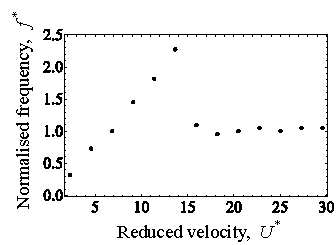
\includegraphics[width=0.38\textwidth]{figs/yStrFreq5}
  \caption{Evolution of the normalised cylinder displacement frequency, $\fstr$, with respect to reduced velocity $\ured$, for the pure cruciform case.}
  \label{fig:yStrFreq5}
\end{figure}

We show the evolution of the normalised cylinder vibration frequency $\fstr$ with respect to $\ured$ in Fig. \ref{fig:yStrFreq5}. Inspecting Fig. \ref{fig:yStrFreq5}, we immediately notice two distinct evolutionary patterns for $\fstr$with a sharp boundary at $\ured = \ursi$. Between $\uron \leq \ured \leq \ursi$, the $\fstr$ trend follows closely the shedding frequency of Karman vortices from an isolated, fixed circular cylinder \citep{Blevins1990}. The Karman vortex shedding frequency is given as an empirical equation in Eq. \ref{eq:karmanSheddingFreq}.

\begin{equation}
  \fvk = 0.198 \left( 1 - \frac{19.7}{\re} \right) DU
  \label{eq:karmanSheddingFreq}
\end{equation}

\noindent Here, $\fvk$, $D$ and $U$ are the vortex shedding frequency, diameter of the isolated circular cylinder and $U$ the freestream velocity respectively. We can easily see how $\fvk$ is a linear function of $U$, and this is what gives rise to the linear pattern of $\fstr$ within $\uron \leq \ured \leq \ursi$. Then, within $\urse \leq \ured \leq \urtt$, $\fstr$ drops close to 1, indicating synchronisation between lift and cylinder vibration. We think this synchronisation is what gives rise to the bigger $\ystr$, compared to $\uron \leq \ured \leq \ursi$.

Inspecting the evolution of \rms{} amplitude of lift coefficient $\clrms$ and the normalised lift coefficient frequency $\fclstr$ with respect to $\ured$ in Fig. \ref{fig:cl90}, provided more evidence supporting the assertion that $\ured = \urse$ is a boudary berween two vibration-driving mechanisms. In fact, the observation at $\urse$ in Fig. \ref{fig:clRMS5} indicates that the SVIV regime is still in its infancy, due to the dip in $\clrms$ at that $\ured$, compared to $\ured = \ursi$. In Fig. \ref{fig:clFreq5}, we also draw a dashed line illustrating $f^{*}_{v} = \fvk/D$, where $\fvk$ is the shedding frequency of Karman vortices from a smooth isolated circular cylinder described in Eq. \ref{eq:karmanSheddingFreq}.

The trend found in $\fclstr$ vs. $\ured$ is very similar to that found in Fig. \ref{fig:yStrFreq5}. We interpret this similarity as an indication of the symmetry of lift produced along the cylinder. Our reasoning stems from the findings of \citet{Zhao2018a}, who revealed how lift is distributed along the upstream cylinder of a two-cylinder \angfi{} cruciform. They did this by computing sectional lift coefficients along the upstream cylinder. This system produces a symmetric distribution of sectional lift coefficient, with $Z = 0$ being the plane of symmetry. An asymmetrical distribution of the sectional lift coefficient may produce a trend in $\yrms$ and $\fstr$ that is dissimilar to those found in $\clrms$ and $\fclstr$, due to the irregular moment acting on the cylinder.

\begin{figure}
  \centering
  \begin{subfigure}[h]{0.38\textwidth}
    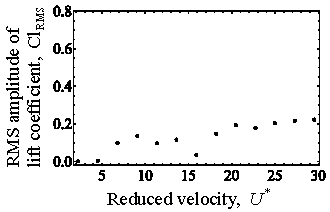
\includegraphics[width=\textwidth]{figs/clRMS5}
    \caption{Evolution of $\clrms$ with respect to $\ured$.}
    \label{fig:clRMS5}
  \end{subfigure}
  \hspace{6mm}
  \begin{subfigure}[h]{0.38\textwidth}
    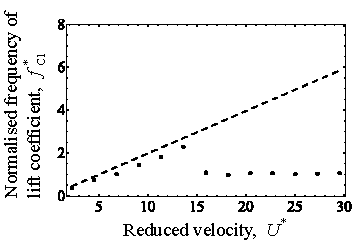
\includegraphics[width=\textwidth]{figs/clFreq5}
    \caption{Evolution of $\fclstr$ with respect to $\ured$}
    \label{fig:clFreq5}
  \end{subfigure}

  \caption{Evolution of the lift coefficient \rms{} amplitude ($\clrms$) and normalised frequency of lift coefficient ($\fclstr$), with respect to reduced velocity $\ured$, for the pure cruciform case. The dashed line in Fig. \ref{fig:clFreq5} visualises the shedding frequency of Karman vortex computed from Eq. \ref{eq:karmanSheddingFreq}.} \label{fig:cl90}
\end{figure}

\subsection{Main vibration-driving vortical structure}\label{ssec:svivRegimeVortStruct}
Recall Figs. \ref{fig:yStrRMS1} and \ref{fig:yStrFreq5}. Out of all thirteen variants of $\ured$ studied in the pure cruciform case, seven within $\urse \leq \ured \leq \urtt$ sustain high-amplitude vibrations with no foreseeable upper limit within our observation window. For a more complete understanding of the mechanism driving the vibration, we need to know what are the vortical structures dominating the flow are and how they interact with each other.

\begin{figure}
  \centering
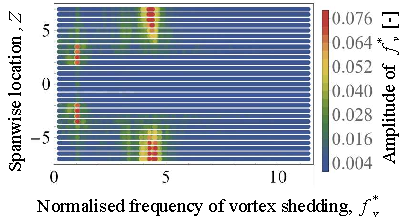
\includegraphics[width=0.48\textwidth]{figs/probe90YU10}
\caption{Distribution of normalised frequency of vortex shedding, along the span of the cylinder of the pure cruciform at $\ured = \urte$.}
  \label{fig:probe90YU10}
\end{figure}

Let us denote coordinates in our simulation domain in the following manner: $\left( X, Y, Z \right) = \left( \frac{x}{D}, \frac{y}{D}, \frac{z}{D} \right)$. We sampled the $y$-component velocity fluctuations on the $\left ( X, Y \right ) = \left ( 1.96, 0 \right )$ line, along the span of the cylinder in $0.5D$ increments, i.e. at coordinates $\left ( 1.96, 0, 7.5 \right )$, $\left ( 1.96, 0, 7.0 \right )$, \dots, $\left ( 1.96, 0, -7.5 \right )$. The distance $X = 1.96$ from the origin is equivalent to $1D$ downstream the trailing edge of the strip plate, and we chose this location as it is not too close to the cruciform that the vortical structures have not fully formed, and not too far, obfuscating meaningful observation of the structures.

The shedding of vortical structures leave their footprint on the flow field in the form of velocity fluctuations. Our choice of analysing the fluctuations of the $y$-component of velocity is made due to the fact that our oscillator is constrained to move only in the transverse direction. Then, we processed the velocity fluctuations with FFT to obtain the Fourier transform of the fluctuation signals at each spanwise location. The combines Fourier transforms are presented using a colour map in Fig. \ref{fig:probe90YU10}. In this figure, every point is a result of that FFT giving us a spatial understanding of the vortical structures present in the flow. The abscissa and ordinates denotes $\fstr$ and $Z$ coordinates respectively, while the bar legend gives the amplitude of the FFT result.

Through inspection, we immediately notice two frequency bands with high amplitudes namely $\fstr \approx 1$ and $\fstr \approx 4.5$. The locations of these bands are between $3 \leq Z \leq 4.5$ for the former and $4.5 < Z \leq 7$ for the latter. Aided with this visualisation, we can give meaning to the $x$ and $z$-components of vorticity visualised in Fig. \ref{fig:vortStruct90} . The slices in Fig. \ref{fig:vortStruct90} visualise the distribution of the $x$ (streamwise) and $z$ (Karman) components of vorticity at the $X = 1.96$ plane. The plane is viewed from downstream (viewer standing at $X = 1.96$, looking towards the cruciform), and we present the vorticites in units of \si{\per\second}. Furthermore, the visualisations are made when the lift coefficient Cl is at a maximum ($\text{Cl}_{\text{max}}$).

Comparing Fig. \ref{fig:probe90YU10} with Fig. \ref{fig:vortStruct90} suggests that the $\fstr \approx 1$ band is actually due to the shedding of streamwise vortex of a scale close to $1D$ while the $\fstr \approx 4.5$ seems to be due to the shedding of Karman vortices. Contrary to the vortical structure commonly observed in studies of isolated circular cylinders \citep{Deng2007,Kinaci2016,Duranay2020}, in the pure cruciform case, two distinct vortical structures take shape in the flow, namely streamwise and Karman vortices. This is consistent with the findings in \citet{Koide2017} or \citet{Zhao2018a}, where they observed a pair of streamwise vortices on a scale of $\approx 1D$ form in the vicinity of the cruciform juncture, and Karman vortices further away in the spanwise direction. Note that the vibration-driving streamwise vortices forming close to the cruciform juncture exist in pairs: in Fig. \ref{fig:vorx90}, we observe one rotate in the clockwise direction when $Z > 0$ and the other in the counter-clockwise direction when $Z < 0$. What results from this counter-rotating vortex pair is a downward thrust, propelling the cylinder upwards, and consistent with the fact that we visualised the vorticity fields when the Cl is at a maximum. We also observe the core of both streamwise vortices lie approximately on the same $Y$-plane, parallel to the axis of the cylinder.

\begin{figure}
  \centering
  \begin{subfigure}[h]{0.28\textwidth}
    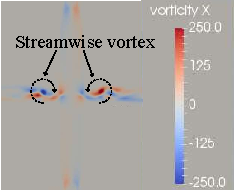
\includegraphics[width=\textwidth]{figs/vorx90}
    \caption{$x$-component vorticity}
    \label{fig:vorx90}
  \end{subfigure}
  \hspace{6mm}
  \begin{subfigure}[h]{0.28\textwidth}
    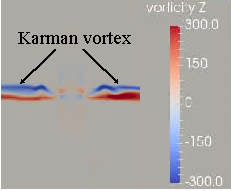
\includegraphics[width=\textwidth]{figs/vorz90}
    \caption{$z$-component vorticity}
    \label{fig:vorz90}
  \end{subfigure}

  \caption{Dominant vortical structures at $\ured = \urte$ observed in the pure cruciform case. The vorticity slices shown are the $x$ and $y$-component vorticities at $x/D = 1.96D$ ($1D$ downstream the trailing edge of strip plate) plane, viewed orthogonal to that plane from downstream. The vorticities have a unit of \si{\per\second}.} \label{fig:vortStruct90}
\end{figure}

\subsection{Phase lag between Cl and $\ystr$} \label{ssec:phaseLag90}

To understand the interplay between lift and cylinder displacement, we compute the phase lag $\plag$ by taking the Hilbert transform of both $\ystr$ and Cl signals, as \citet{Khalak1999} did in their VIV study of isolated circular cylinders. However, since Hilbert transform only produce physically meaningful results when used on monocomponent signals \citep{Huang1998,Huang2005,Huang2014}, the signals first needs to be decomposed into components that satisfy the aforementioned condition, referred to in the literature as the intrinsic mode function (IMF). To achieve this, we implement the ensemble empirical mode decomposition (EEMD) \citep{Wu2008}.

The word ``ensemble'' in EEMD refers to the fact that it is an adaptation of the empirical mode decomposition (EMD) algorithm that takes the ensemble average of $n$-variants of the same IMF. The method outlined by the original authors of EEMD \citep{Wu2008} to produce $n$-variants of the same IMF is by producing $n$ white noise signals of equal length to the signal being decomposed, with an amplitude 10\% to 20\% the amplitude of the standard deviation of the original signal. Then, we add the $n$-number of white noise signals to the signal being decomposed, creating $n$-variants of the original signal. Each variant is then decomposed according to the following rule:

\begin{enumerate} \label{enumerate:emd}
  \item Connect all the signal maxima/minima with cubic splines, thus obtaining the signal envelope. \label{enum:envelope}
  \item Determine the local mean of the envelope for the span of the data. \label{enum:localMean}
  \item Compute the difference between the local mean of the envelope and the original data. \label{enum:difference}
  \item Repeat steps \ref{enum:envelope} and \ref{enum:localMean} on the difference computed in \ref{enum:difference} until we obtain an our first IMF (IMF 1). \label{enum:imf}
  \item Subract IMF 1 from the original signal and we are left with the remainder of the signal, upon which steps \ref{enum:envelope} to \ref{enum:imf} are repeated, producing IMF 2, IMF 3 and so on until we are left with what is called the residual of the original signal, from which no more IMF can be extracted.

\end{enumerate}

\noindent Since we constructed $n$-variants of the signal earlier, we effectively have, through the EMD algorithm described, derived $n$-variants of IMF 1, IMF 2 and so on. The ensemble part of EEMD now comes to play, when we averaged all $n$-variants of IMF 1, IMF 2, etc., giving us the ensemble version of each IMF. These are the IMFs that we use in our Hilbert transform. In this work, we produced 150 variants of the original signals using white noises 20\% the amplitude of the standard deviation of the original signal.

\begin{figure}
  \centering
  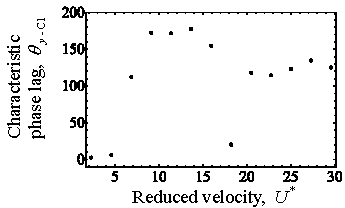
\includegraphics[width=0.4\textwidth]{figs/phaseLag5}
  \caption{Phase lag $\plag$ (\si{\degree}) between Cl and $\ystr$ when \angfi{}.}
  \label{fig:phaseLag90deg}
\end{figure}

Once the IMF components are retrieved, we compute the instantaneous phase of the IMFs $C_{1},C_{2},\dots,C_{i}$ by constucting an analytical signal $z \left( t \right)$ from them in the following manner. First we compute the Hilbert transform of the IMF, $H_{i}$ (see Eq. \ref{eq:hilbertTransform}),

\begin{equation}
  H_{i} \left( t \right) = \frac{1}{\pi} \text{PV} \int\limits_{}^{\infty} \frac{C_{i} \left( \tau \right)}{t - \tau} d\tau,
  \label{eq:hilbertTransform}
\end{equation}

\noindent where PV means the Cauchy principal value. Then, we construct $z \left( t \right)$ as shown in Eq. \ref{eq:analiticalSignal}.

\begin{equation}
  z \left( t \right) = C_{i} \left( t \right) + i H_{i} \left( t \right) = a(t) \cdot e^{i \; \theta(t)}.
  \label{eq:analiticalSignal}
\end{equation}

\noindent The $i$ in Eq. \ref{eq:analiticalSignal} represents the complex number. In the exponent form of $z \left( t \right)$, $a(t) = \sqrt{C^{2}_{i} \left( t \right) + H^{2}_{i} \left( t \right)}$ and $\theta (t) = \arctan \left( H_{i}/C_{i} \right)$ describes the instantaneous amplitude and phase of the IMF, respectively. The lift coefficient Cl and the cylinder displacement $y$ each has their own instantaneous phases $\theta_{\text{Cl}}(t)$ and $\theta_{y}(t)$. The characteristic phase lag $\plag$ is thus defined such that

\begin{equation}
  \plag = \frac{1}{T} \int_{0}^{T} \left[ \theta_{\text{Cl}}(t) - \theta_{y}(t) \right] dt.
  \label{eq:phaseLagDefinition}
\end{equation}

Out of $C_{i}$ IMFs for each of $\ystr$ and Cl, we select the ones for computation of instantaneous phase according to the following rule. First, we choose the IMF component of $\yrms$ with the largest \rms{} amplitude to represent the original $\ystr$ signal. Then, we choose the component of Cl with the highest correlation to the IMF component of $\ystr$, to represent the Cl signal. The degree of correlation is determined by computing the cross-correlation between the two.

The characteristic phase angle $\plag$ defined in Eq. \ref{eq:phaseLagDefinition} is what we summarise against $\ured$ in Fig. \ref{fig:phaseLag90deg}. Note that the $\plag$ pattern between $0 \leq \ured \leq \ursi$ resembles that which is found in isolated cylinder systems undergoing KVIV. We also observe that $\plag$ starts to drop when $\ured = \urse$, supporting the view that a fundamental change in vibration-driving mechanism took place at that $\ured$, culminating in the emergence of the initial branch for SVIV at $\ured = \urei$.

\section{Transition to Karman vortex-driven vibration}\label{sec:transitionToKarman}
\subsection{The amplitude and frequency response}\label{ssec:transRegimeAmpFreqResp}

As we reduce the cruciform angle to \angfo{} and \angth{}, we find that the SVIV branch observed in the pure cruciform case as $\ured \geq \urse$ disappear, as one can inspect in Fig. \ref{fig:yStrRMS23}. For the \angth{} cruciform, even $\yrms$ at the KVIV upper branch ($\ured = \urtw$) is lower than the corresponding values for both the \angfi{} and \angfo{} cruciforms.

\begin{figure}
  \centering
  \begin{subfigure}[h]{0.4\textwidth}
    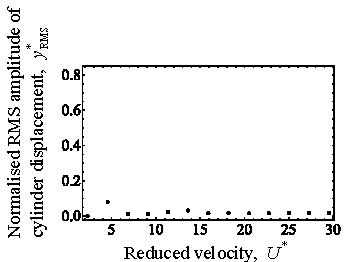
\includegraphics[width=\textwidth]{figs/yStrRMS2}
  \caption{The \angfo{} cruciform.}
    \label{fig:yStrRMS2}
  \end{subfigure}
  \hspace{6mm}
  \begin{subfigure}[h]{0.4\textwidth}
    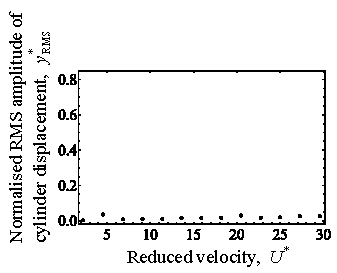
\includegraphics[width=\textwidth]{figs/yStrRMS3}
    \caption{The \angth{} cruciform.}
    \label{fig:yStrRMS3}
  \end{subfigure}

  \caption{Evolution of the normalised \rms{} amplitude of cylinder displacement $\yrms$, with respect to reduced velocity $\ured$, for the \angfo{} and \angth{} cruciform.}
  \label{fig:yStrRMS23}
\end{figure}

Another striking departure from the trend observed in the pure cruciform case, can be found in the evolution of $\fstr$ in Fig. \ref{fig:yStrFreq43}. For the \angfo{} cruciform in Fig. \ref{fig:yStrFreq4}, $\fstr$ seems to fluctuate with respect to $\ured$ - suggesting asymmetry in the vortical structures regulating the vibration as discussed previously in \S\ref{ssec:svivRegimeAmpFreqResp}. This fluctuation is however, not as pronounced in Fig. \ref{fig:yStrFreq3}, compared to Fig. \ref{fig:yStrFreq4}. We think this behaviour is due to the \angth{} cruciform being less similar to the \angfi{} cruciform, in contrast to \angfo{}. In other words, the \angth{} cruciform is less in transition from the response of the \angfi{} cruciform and the flow around it is more evolved into its new configuration, unlike the \angfo{} cruciform.

\begin{figure}
  \centering
  \begin{subfigure}[h]{0.4\textwidth}
    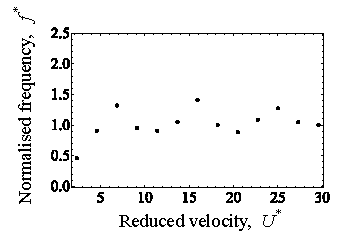
\includegraphics[width=\textwidth]{figs/yStrFreq4}
    \caption{The \angfo{} cruciform.}
    \label{fig:yStrFreq4}
  \end{subfigure}
  \hspace{6mm}
  \begin{subfigure}[h]{0.4\textwidth}
    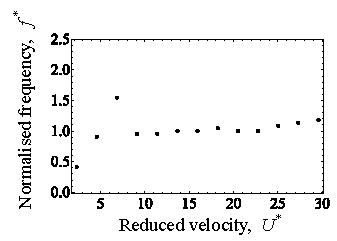
\includegraphics[width=\textwidth]{figs/yStrFreq3}
    \caption{The \angth{} cruciform.}
    \label{fig:yStrFreq3}
  \end{subfigure}

  \caption{Evolution of the normalised cylinder displacement frequency, $\fstr$, with respect to reduced velocity $\ured$, for the \angfo{} and \angth{} cruciforms.}
  \label{fig:yStrFreq43}
\end{figure}

We summarised the \rms{} lift coefficients $\clrms$ of the \angfo{} and \angth{} cruciforms in Fig. \ref{fig:clRMS43}. Here, we find that their evolution with respect to $\ured$ in Figs. \ref{fig:clRMS4} and \ref{fig:clRMS3} approximates their corresponding $\yrms$ trend in Figs. \ref{fig:yStrRMS2} and \ref{fig:yStrRMS3}. As for the variation of $\fclstr$ with respect to $\ured$, for both the \angfo{} and \angth{} cruciforms, both exhibit outstanding similarity to $\fvk$ of Eq. \ref{eq:karmanSheddingFreq}. This trait hints that vibrations resulting from the \angfo{} and \angth{} cruciforms are primarily regulated by the shedding of Karman vortices.

The fact that the $\fclstr$ trends observed in Figs. \ref{fig:clFreq4} and \ref{fig:clFreq3} do not lead to similar trends in the evolution of $\fstr$ in Figs. \ref{fig:yStrFreq4} and \ref{fig:yStrFreq3} leads us to believe there is something more fundamental at play in developing the $\fstr$ patterns we observed. Hence we examined the vortical structures present in the flow surrounding the \angfo{} and \angth{} cruciforms, and discuss our findings in \S\ref{ssec:transitionalRegimeVortStruct}. 

\begin{figure}
  \centering
  \begin{subfigure}[h]{0.4\textwidth}
    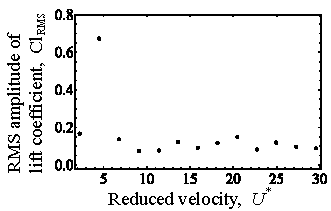
\includegraphics[width=\textwidth]{figs/clRMS4}
    \caption{The \angfo{} cruciform.}
    \label{fig:clRMS4}
  \end{subfigure}
  \hspace{6mm}
  \begin{subfigure}[h]{0.4\textwidth}
    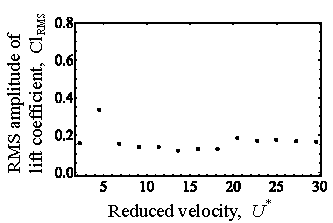
\includegraphics[width=\textwidth]{figs/clRMS3}
    \caption{The \angth{} cruciform.}
    \label{fig:clRMS3}
  \end{subfigure}

  \caption{Evolution of the normalised Cl \rms{} amplitude, $\clrms$, with respect to reduced velocity $\ured$, for the \angfo{} and \angth{} cruciforms.}
  \label{fig:clRMS43}
\end{figure}

\begin{figure}
  \centering
  \begin{subfigure}[h]{0.4\textwidth}
    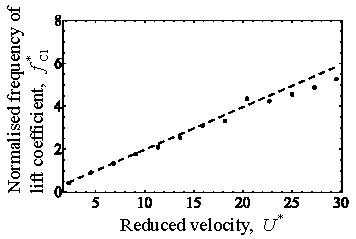
\includegraphics[width=\textwidth]{figs/clFreq4}
    \caption{The \angfo{} cruciform.}
    \label{fig:clFreq4}
  \end{subfigure}
  \hspace{6mm}
  \begin{subfigure}[h]{0.4\textwidth}
    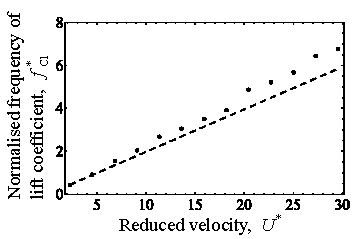
\includegraphics[width=\textwidth]{figs/clFreq3}
    \caption{The \angth{} cruciform.}
    \label{fig:clFreq3}
  \end{subfigure}

  \caption{Evolution of the normalised Cl frequency, $\fclstr$, with respect to reduced velocity $\ured$, for the \angfo{} and \angth{} cruciforms. The dashed lines outline $\fvk$ from Eq. \ref{eq:karmanSheddingFreq}.} \label{fig:clFreq43}
\end{figure}

\subsection{Main vibration-driving vortical structure}\label{ssec:transitionalRegimeVortStruct}
As the first step, we computed the FFT of the $y$-component of velocity similar to what we did in Fig. \ref{fig:probe90YU10} for both the \angfo{} and \angth{} cruciforms. Our initial assesment of the $\fvkstr$ distribution along the cylinder axis in Figs. \ref{fig:probe675YU10} and \ref{fig:probe45YU10} is that there is a strong representation of the Karman shedding frequency in both cases, which at $\ured = \urte$ is $\fvkstr = 4.49$. However, unlike Fig. \ref{fig:probe90YU10}, there is no frequency band close to 1 around the cruciform juncture.

Our first guess is that streamwise vortices driving the vibration in the pure cruciform case do not get initiated once the cruciform angle deviates away from \angfi{}. However, $x$ and $z$-component vorticity visualisations in Fig. \ref{fig:vortStruct67545} points out otherwise. These visualisations are produced under the same conditions as Fig. \ref{fig:vortStruct90}. Inspecting Figs. \ref{fig:vorx675} and \ref{fig:vorx45}, we can quite clearly make out the large-scale streamwise vortices close to the cruciform juncture. We thus expect the cylinder vibration and streamwise vortices to synchronise to each other, resulting in an $\fstr \approx 1$ accross the values of $\ured$ after the lower branch of KVIV, which appears at $\ured = \urth$. In addition, we expect there to be a large amplitude response from the cylinder due to the formation and sustenance of the streamwise vortices close to the cruciform juncture. This was not the case.

We think the reason behind this lies in the distribution of the streamwise vortex cells along the cylinder axis. As we mentioned in \S\ref{ssec:svivRegimeVortStruct}, the streamwise vortex pair in the pure cruciform case lie on a plane parallel to the axis of the cylinder. The shared plane of formation parallel to cylinder axis is what we think as key to the large amplitude response observed in the pure cruciform case. A formation plane parallel to the cylinder axis ensures the resulting downward thrust to act perpendicular to the cylinder, securing a larger amplitude response. Also, the streamwise vortex cell on each side of the $Z = 0$ plane must be of opposing rotational direction for the production of thrust. We find these two aspects missing in the \angfo{} and \angth{} cruciforms in Fig. \ref{fig:vortStruct67545}.

What takes place in Figs. \ref{fig:vorx675} and \ref{fig:vorx45} is, two streamwise vortex cells of opposing poles form on each side of the $Z = 0$ plane. The result of this vortical arrangement is severe diminishing of useful thrust, and by extension, lift acting on the cylinder. This explains why the amplitude of $\fvstr$ at and within the vicinity of $1$ is extremely small in comparison to the dominant band close to $\fvkstr = 4.49$, resulting in a low amplitude response for most of the $\ured$ studied, even when $\fstr \approx 1$.

We also managed to find the source of asymmetry in the vortical structure distribution around the cruciform, which becomes apparent upon closer comparison of Fig. \ref{fig:vorz675} and Fig. \ref{fig:vorz45}. The Karman vortices of the \angfo{} cruciform are shed at different phases depending on which side of the $Z = 0$ plane we are observing. For the particular case in Fig. \ref{fig:vorz675}, Karman vortices are being shed from the top of the cylinder when $Z < 0$, and from the bottom of the cylinder when $Z > 0$. What suggested this interpretation is our observation of a strong expression of $-z$ vorticity when $Z < 0$ from the top of the cylinder, while on the $Z > 0$ half of our domain is a strong expression of $+z$ vorticity from the bottom of the cylinder. We do not see this take place in Fig. \ref{fig:vorz45}. On both sides of the $Z = 0$ plane, we note the strong expression of $-z$ vorticity from the top of the cylinder. This asymmetry leads to competing vibration-driving mechanisms resulting in the oscillatory behaviour of $\fstr$ seen in Fig. \ref{fig:yStrFreq4}.

\begin{figure}
  \centering

  \begin{subfigure}[h]{0.46\textwidth}
    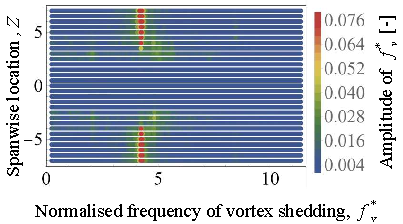
\includegraphics[width=\textwidth]{figs/probe675YU10}
    \caption{The $\fvstr$ for the \angfo{} cruciform.}
    \label{fig:probe675YU10}
  \end{subfigure}
  \hspace{6mm}
  \begin{subfigure}[h]{0.46\textwidth}
    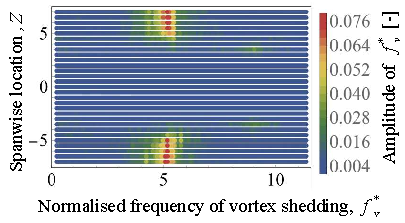
\includegraphics[width=\textwidth]{figs/probe45YU10}
    \caption{The $\fvstr$ for the \angth{} cruciform.}
    \label{fig:probe45YU10}
  \end{subfigure}

  \caption{Distribution of normalised frequency of vortex shedding, along the span of the cylinder of the \angfo{} and \angth{} cruciforms at $\ured = \urte$.}
  \label{fig:probe67545YU10}
\end{figure}

\begin{figure}
  \centering
  \begin{subfigure}[h]{0.4\textwidth}
    \centering
    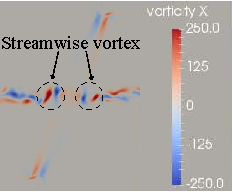
\includegraphics[width=0.7\textwidth]{figs/vorx675}
    \caption{$x$-component vorticity, \angfo{} cruciform.}
    \label{fig:vorx675}
  \end{subfigure}
  \begin{subfigure}[h]{0.4\textwidth}
    \centering
    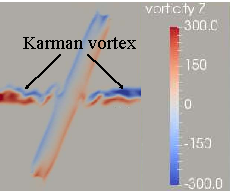
\includegraphics[width=0.7\textwidth]{figs/vorz675}
    \caption{$z$-component vorticity, \angfo{} cruciform.}
    \label{fig:vorz675}
  \end{subfigure}

  \begin{subfigure}[h]{0.4\textwidth}
    \centering
    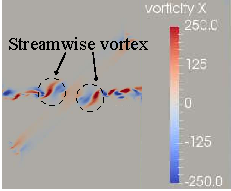
\includegraphics[width=0.7\textwidth]{figs/vorx45}
    \caption{$x$-component vorticity, \angth{} cruciform.}
    \label{fig:vorx45}
  \end{subfigure}
  \begin{subfigure}[h]{0.4\textwidth}
    \centering
    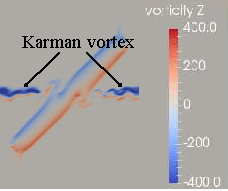
\includegraphics[width=0.7\textwidth]{figs/vorz45}
    \caption{$z$-component vorticity, \angth{} cruciform.}
    \label{fig:vorz45}
  \end{subfigure}

  \caption{Dominant vortical structures at $\ured = \urte$ observed in the \angfo{} and \angth{} cases. The vorticity slices shown are the $x$ and $y$-component vorticities (\si{\per\second}) at the $x/D = 1.96D$ plane, viewed orthogonal to that plane from downstream.} \label{fig:vortStruct67545}
\end{figure}

\subsection{Phase lag between Cl and $\ystr$} \label{ssec:phaseLag67545}
Evolution of $\plag$ for the \angfo{} and \angth{} cruciforms share a similar trend in the $\uron \leq \ured \leq \urth$ range. For the \angfo{} cruciform, past $\ured = \urth$, there seem to be two distinct VIV branches between $\uron \leq \ured \leq \ursi$, and between $\urse \leq \ured \leq \urtt$. In the first branch between $\uron \leq \ured \leq \ursi$, $\plag$ seems to remain close to \SI{70}{\degree}, while in the second branch, close to \SI{110}{\degree}. In some sense, this is fairly similar to the $\plag$ vs. $\ured$ pattern of the pure cruciform case, except for two features. First, the lower branch of KVIV -- which in the pure cruciform case exhibits a $\plag \approx \SI{180}{\degree}$ -- does not extend beyond $\ured = \urth$. Instead, the value for $\plag$ suddenly drops to $\approx \SI{70}{\degree}$ before jumping back up to $\approx \SI{110}{\degree}$ starting at $\ured = \urse$. This value of \SI{110}{\degree} is curiously close to $\plag$ of the pure cruciform between $\urni \leq \ured \leq \urtt$, equivalent to the upper branch of SVIV. If we work backwards from $\ured = \urni$ in the direction of decreasing $\ured$, and compare Fig. \ref{fig:phaseLag675deg} and Fig. \ref{fig:phaseLag90deg}, we confront the possibility that the $\plag = \SI{70}{\degree}$ branch of the \angfo cruciform is a \textit{variant} of the SVIV initial branch. For the pure cruciform case, this occurs within a narrow window of $\urse < \ured < \urni$, with $\plag \approx \SI{20}{\degree}$.

For the \angth{} cruciform in Fig. \ref{fig:phaseLag45deg}, right after lower branch of KVIV at $\ured = \urth$, $\plag$ transitioned to $\approx \SI{65}{\degree}$ between $\urfi \leq \ured \leq \urni$. The proximity between the values \SI{65}{\degree} and \SI{70}{\degree} for the \angfo{} cruciform suggests the equivalence of the two branches. However, we are inclined to a more cautious conclusion: the two are \textit{variants} of the same branch that is only similar in limited respects as they originate from different angled cruciforms. In this respect, the \angth{} cruciform is much less similar to the pure cruciform case, as one might expect, simply because \angth{} is a much larger deviation from \angfi{} compared to \angfo{}. This larger deviation is in our opinion what causes $\plag$ in the \angth{} case to drop further to $\approx \SI{35}{\degree}$ within $\urte \leq \ured \leq \urtt$, instead of jumping up to some mean value between $100 \leq \plag \; (\si{\degree}) \leq 130$ similar to what we observe in the \angfi{} and \angfo{} cruciforms.

\begin{figure}
  \centering
  \begin{subfigure}[h]{0.4\textwidth}
    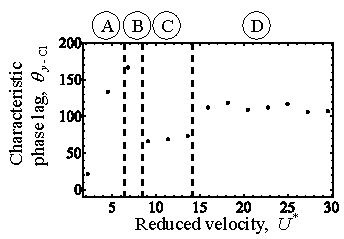
\includegraphics[width=\textwidth]{figs/phaseLag4}
    \caption{Phase lag for the \angfo{} cruciform.}
    \label{fig:phaseLag675deg}
  \end{subfigure}
  \hspace{6mm}
  \begin{subfigure}[h]{0.4\textwidth}
    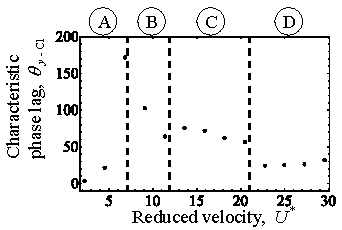
\includegraphics[width=\textwidth]{figs/phaseLag3}
    \caption{Phase lag for the \angth{} cruciform.}
    \label{fig:phaseLag45deg}
  \end{subfigure}

  \caption{Phase lag $\plag$ (\si{\degree}) between Cl and $\ystr$ when \angfo{} and \angth{}.}
  \label{fig:phaseLag67545deg}
\end{figure}

\section{Karman vortex-driven vibration}\label{sec:kvivRegime}
\subsection{The amplitude and frequency response}\label{ssec:kvivAmpFreqResp}
As we decrease the cruciform angle even further to \angtw{}, we observe a significant change in the amplitude and frequency response, compared to the steep-angled cruciform previously explored in \S\ref{sec:transitionToKarman}. Consider Figs. \ref{fig:yStrRMS4} and \ref{fig:yStrFreq2}. There is no apparent KVIV upper branch similar to what we have seen in Figs. \ref{fig:yStrRMS2} and \ref{fig:yStrFreq4} at $\ured = \urtw$. Then, we observe no significant vibration elicited from the oscillator until $\ured = \urni$. When $\ured = \urni$, there is a abrupt jump in $\yrms$ from $\yrms < 0.02$ to $\yrms \approx 0.3$. The $\fstr$ vs. $\ured$ trend demonstrated a bypassing of the KVIV lower branch - which occurred at $\ured = \urth$ in the steep-angled cruciform of \S\ref{sec:transitionToKarman} - right into $\fstr \approx 1$. Past $\ured = \urni$, the value for $\yrms$ continues to increase and saturates at $\ured = \urel$, and $\fstr$ continues to be close to $1$ up to $\ured = \urtt$.

The \angon{} cruciform (Figs. \ref{fig:yStrRMS5}, \ref{fig:yStrFreq1}) in essence exhibits a very similar trend in its $\yrms$ and $\fstr$ evolutions with respect to $\ured$. However, the jump -- which for the \angtw{} cruciform occurs at $\ured = \urni$ -- occurs at a a much lower $\ured = \urfo$. Then, $\yrms$ continues to grow until $\ured = \urni$, reaching a staggering $\yrms \approx 0.8$, a value no other study on energy harvesting using cruciform oscillators has ever achieved. The value of $\yrms$ then saturates close to $0.8$ up to $\ured = \urtt$. Also similar to the \angtw{} cruciform, $\fstr$ falls close to $1$ at same $\ured$ the $\yrms$ jump occurs - hinting at synchronisation between vortex shedding and system natural frequency.

\begin{figure}
  \centering
  \begin{subfigure}[h]{0.4\textwidth}
    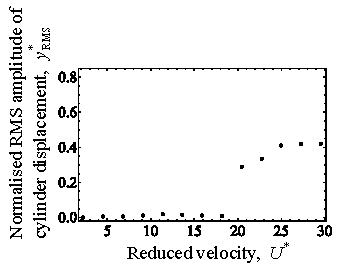
\includegraphics[width=\textwidth]{figs/yStrRMS4}
  \caption{The \angtw{} cruciform.}
    \label{fig:yStrRMS4}
  \end{subfigure}
  \hspace{6mm}
  \begin{subfigure}[h]{0.4\textwidth}
    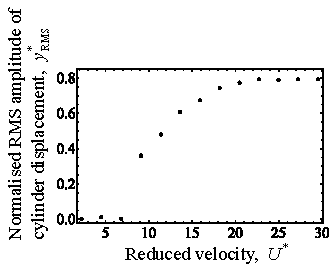
\includegraphics[width=\textwidth]{figs/yStrRMS5}
    \caption{The \angon{} cruciform.}
    \label{fig:yStrRMS5}
  \end{subfigure}

  \caption{Evolution of the normalised \rms{} amplitude of cylinder displacement $\yrms$, with respect to reduced velocity $\ured$, for the \angtw{} and \angon{} cruciform.}
  \label{fig:yStrRMS45}
\end{figure}

\begin{figure}
  \centering
  \begin{subfigure}[h]{0.4\textwidth}
    \includegraphics[width=\textwidth]{figs/yStrFreq2}
    \caption{The \angtw{} cruciform.}
    \label{fig:yStrFreq2}
  \end{subfigure}
  \hspace{6mm}
  \begin{subfigure}[h]{0.4\textwidth}
    \includegraphics[width=\textwidth]{figs/yStrFreq1}
    \caption{The \angon{} cruciform.}
    \label{fig:yStrFreq1}
  \end{subfigure}

  \caption{Evolution of the normalised cylinder displacement frequency, $\fstr$, with respect to reduced velocity $\ured$, for the \angtw{} and \angon{} cruciforms.}
  \label{fig:yStrFreq21}
\end{figure}
Apart from the amplitude/frequency response of the \angtw{} cruciform, the evolution of $\clrms$ against $\ured$ showcases a similar trend to the evolution $\yrms$, as shown in Fig. \ref{fig:clRMS2}. The corresponding $\fclstr$ in Fig. \ref{fig:clFreq2} demonstrates the dominant frequency of Cl taking after Eq. \ref{eq:karmanSheddingFreq} between $\uron \leq \ured \leq \urei$, before abruptly dropping close to $1$ between $\urni \leq \ured \leq \urtt$. This in part informs us that the flow between $\uron \leq \ured \leq \urei$ is governed by flow physics that are similar to both \angfo{} and \angth{} within the same $\ured$ range.

For the \angon{} cruciform, we see that the jump in $\clrms$ occurs at the same $\ured$ as the jump in the corresponding $\yrms$ i.e., $\ured = \urfo$. After $\ured = \urfo$, the magnitude of $\clrms$ gradually drops to a final value of $\clrms \approx 0.45$ at $\ured = \urni$, and remains there up to $\ured = \urtt$. Similar to the \angtw{} cruciform, $\fclstr$ grows linearly in accordance with, again, Eq. \ref{eq:karmanSheddingFreq} until the jump in both $\clrms$ and $\yrms$, where $\fclstr$ drops close to $1$ for the rest the $\ured$ we examine in this study.

\begin{figure}
  \centering
  \begin{subfigure}[h]{0.4\textwidth}
    \includegraphics[width=\textwidth]{figs/clRMS2}
    \caption{The \angtw{} cruciform.}
    \label{fig:clRMS2}
  \end{subfigure}
  \hspace{6mm}
  \begin{subfigure}[h]{0.4\textwidth}
    \includegraphics[width=\textwidth]{figs/clRMS1}
    \caption{The \angon{} cruciform.}
    \label{fig:clRMS1}
  \end{subfigure}

  \label{fig:clRMS21}
  \caption{Evolution of the normalised Cl \rms{} amplitude, $\clrms$, with respect to reduced velocity $\ured$, for the \angtw{} and \angon{} cruciforms.}
\end{figure}

\begin{figure}
  \centering
  \begin{subfigure}[h]{0.4\textwidth}
    \includegraphics[width=\textwidth]{figs/clFreq2}
    \caption{The \angtw{} cruciform.}
    \label{fig:clFreq2}
  \end{subfigure}
  \hspace{6mm}
  \begin{subfigure}[h]{0.4\textwidth}
    \includegraphics[width=\textwidth]{figs/clFreq1}
    \caption{The \angon{} cruciform.}
    \label{fig:clFreq1}
  \end{subfigure}

  \label{fig:clFreq21}
  \caption{Evolution of the normalised Cl frequency, $\fclstr$, with respect to reduced velocity $\ured$, for the \angtw{} and \angon{} cruciforms. The dashed lines outline $\fvk$ from Eq. \ref{eq:karmanSheddingFreq}.}
\end{figure}


\subsection{Main vibration-driving vortical structure}\label{ssec:kvivRegimeVortStruct}
To understand the cause behind the marked difference between the amplitude/frequency response in both \angfo{} and \angth{} cruciforms, we proceed to deduce the type of vortical structures that form in the flows around the \angtw{} and \angon{} cruciform. We first produce the visualise of $\fvstr$ along the cylinder, in the same manner as Figs. \ref{fig:probe90YU10} and \ref{fig:probe67545YU10}, in Fig. \ref{fig:probe225YU10}. Inspecting Fig. \ref{fig:probe225YU10}, we immediately notice that several frequency bands exist: $\fvstr \approx 1,\, 2,\, 3,\, 4.5$, the most visible of which is the $\fvstr \approx 1$ band. However, unlike the pure cruciform case in Fig. \ref{fig:probe90YU10} -- where the dominant frequency bands are localised to certain regions along the cylinder -- the $\fvstr \approx 1$ band of the \angtw{} cruciform seems to encompass the length of the cylinder. This also seems to be the case for the \angon{} cruciform, displaying a dominant $\fvstr$ band at approximately $1$ along the length of the cylinder.

We then queried the $x$ and $z$-component vorticity contours of the \angtw{} cruciform for deeper insight, presented in Figs. \ref{fig:vorx225} and \ref{fig:vorz225}. In doing so, we found that the large scale streamwise vortex pair near the cruciform juncture is absent. Instead, we noticed streamwise vortex cells distributed on both sides of the $Z = 0$ plane, except within the immediate neighbourhood of the cruciform juncture. We note that these streamwise vortex cells are distributed at a slight angle relative to the $z$-axis, seemingly following the angle of the strip plate, i.e. \SI{22.5}{\degree}. Visualisation of the $z$-component vorticity in Fig. \ref{fig:vorz225} intimates the nature of the tilted streamwise vortex cells: they are simply three-dimensional Karman vortex structures, akin to those observed in the experiments of \citet{Williamson1996}, especially mode B. We inferred this from comparison of the same visual region delimited by dashed rectangles in Figs. \ref{fig:vorx225} and \ref{fig:vorz225}, showing the overlap between the streamwise vortex cells and the strong Karman vortex component.

\begin{figure}
  \centering

  \begin{subfigure}[h]{0.46\textwidth}
    \includegraphics[width=\textwidth]{figs/probe225YU10}
    \caption{The $\fvstr$ for the \angtw{} cruciform.}
    \label{fig:probe225YU10}
  \end{subfigure}
  \hspace{6mm}
  \begin{subfigure}[h]{0.46\textwidth}
    \includegraphics[width=\textwidth]{figs/probe00YU10}
    \caption{The $\fvstr$ for the \angon{} cruciform.}
    \label{fig:probe00YU10}
  \end{subfigure}

  \caption{Distribution of normalised frequency of vortex shedding, along the span of the cylinder of the \angtw{} and \angon{} cruciforms at $\ured = \urte$.}
  \label{fig:probe22500YU10}
\end{figure}

\begin{figure}
  \centering
  \begin{subfigure}[h]{0.4\textwidth}
    \centering
    \includegraphics[width=0.7\textwidth]{figs/vorx225}
    \caption{$x$-component vorticity, \angfo{} cruciform.}
    \label{fig:vorx225}
  \end{subfigure}
  \begin{subfigure}[h]{0.4\textwidth}
    \centering
    \includegraphics[width=0.7\textwidth]{figs/vorz225}
    \caption{$z$-component vorticity, \angfo{} cruciform.}
    \label{fig:vorz225}
  \end{subfigure}

  \begin{subfigure}[h]{0.4\textwidth}
    \centering
    \includegraphics[width=0.7\textwidth]{figs/vorx00}
    \caption{$x$-component vorticity, \angth{} cruciform.}
    \label{fig:vorx00}
  \end{subfigure}
  \begin{subfigure}[h]{0.4\textwidth}
    \centering
    \includegraphics[width=0.7\textwidth]{figs/vorz00}
    \caption{$z$-component vorticity, \angth{} cruciform.}
    \label{fig:vorz00}
  \end{subfigure}

  \caption{Dominant vortical structures at $\ured = \urte$ observed in the \angtw{} and \angon{} cases. The vorticity slices shown are the $x$ and $y$-component vorticities (\si{\per\second}) at the $x/D = 1.96D$ plane, viewed orthogonal to that plane from downstream.} \label{fig:vortStruct22500}
\end{figure}

For the \angon{} cruciform in Figs. \ref{fig:vorx00} and \ref{fig:vorz00}, this overlap between the streamwise vortex cells and the distinct Karman vortex component is even more visually pronounced. We interpret this as further evidence to the hypothesis that three-dimensional Karman vortical structures govern the vibration of the cylinder for shallow angled cruciforms, including the \SI{0}{\degree} cruciform, which perhaps is more aptly named in-tandem configuration. Notice that for the \angon{} layout, both the streamwise vortex cells and the Karman vortical structure are arranged parallel to the $z$-axis, or at \SI{0}{\degree} relative to the cylinder. This observation seems to demonstrate the role of the strip plate in shallow angled cruciforms: it modifies the spatial distribution of the Karman vortical structure that is driving the vibration of the cylinder.

As we have seen in \S\ref{sec:svivRegime} and \ref{sec:transitionToKarman}, eliciting a significant vibration amplitude Karman vortex shedding is limited to a narrow $\ured$ range containing the upper branch of KVIV. Beyond that, Karman vortex shedding fails to lock into the natural frequency of the system to produce meaningful vibrations. The fact that shallow angled cruciforms in this \S\ref{ssec:kvivRegimeVortStruct} are able to produce very large vibration amplitudes intimate the crucial role played by the strip plate in forcing the shedding of vortical structures and cylinder vibration to lock into the natural frequency of the system $\fn$. We think the mechanics of this forced lock-in is as follows.

\begin{enumerate}
  \item Shallow angled cruciforms have a larger overlap area between the cylinder and strip plate. This permits a more perceptible interaction among vortices shed from the cylinder and the strip plate.
  \item Upon exceeding a critical $\ured$, vortical structures shed from both the cylinder and the strip plate becomes sufficiently energised, and they start to behave as one.
  \item This vortical synchronisation locks into the natural frequency of the elastic structure in its immediate vicinity - our circular cylinder.
\end{enumerate}

\noindent The results also suggest the total cylinder-strip plate area overlap as a factor influencing the exact $\ured$ at which the vortical synchronisation occurs. The $\ured$ at which the synchronisation -- and the jump to large $\yrms$ amplitude -- occurs at a lower value when the overlap area is bigger. Nevertheless, there seems to be a limit to this lowering of $\ured$, which in this work we determined to be $\ured = \urfo$. Recall that this is the value where the synchronisation begins for the \angon{} layout; the layout where the totality of the cylinder and strip plate projections onto the $y-z$ plane coincides with each other.

\subsection{Phase lag between Cl and $\ystr$} \label{ssec:phaseLag22500}
In Fig. \ref{fig:phaseLag225deg}, we summarise the evolution of $\plag$ with respect to $\ured$ for the \angtw{} cruciform and find $\plag \approx \SI{115}{\degree}$ at $\ured = \urtt$. The significance of $\ured = \urtt$ for the \angtw{} cruciform is that it is where a jump in $\plag$ occurs from $\approx \SI{30}{\degree}$ to $\approx \SI{115}{\degree}$. This abrupt jump usually demarcates transition to the KVIV lower branch, as stated in the discussion accompanying Figs. \ref{fig:phaseLag90deg} and \ref{fig:phaseLag67545deg}, with a value that is very close to \SI{180}{\degree}. The $\plag$ for the \angtw{} cruciform however, is about 36\% smaller than the expected $\approx \SI{180}{\degree}$. This may be the cause of absence of the KVIV lower branch in the $\fstr$ vs. $\ured$ plot of the \angtw{} cruciform (Fig. \ref{fig:yStrFreq2}).

The \angon{} arrangement produces a similar trend to Fig. \ref{fig:phaseLag225deg}, as one can see in Fig. \ref{fig:phaseLag00deg}. However, the $\plag$ jump at  $\ured =\urtt$ is more pronounced and achieves a value very close to \SI{180}{\degree}. Following the sudden jump is the sudden drop at $\ured = \urfo$, which brings $\plag$ to approximately \SI{25}{\degree}. This trend continues up to $\ured = \urse$, after which we find $\plag$ to monotonically increase up to $\ured = \urtt$.

\begin{figure}
  \centering
  \begin{subfigure}[h]{0.4\textwidth}
    \includegraphics[width=\textwidth]{figs/phaseLag2}
    \caption{Phase lag for the \angtw{} cruciform.}
    \label{fig:phaseLag225deg}
  \end{subfigure}
  \hspace{6mm}
  \begin{subfigure}[h]{0.4\textwidth}
    \includegraphics[width=\textwidth]{figs/phaseLag1}
    \caption{Phase lag for the \angon{} cruciform.}
    \label{fig:phaseLag00deg}
  \end{subfigure}

  \caption{Phase lag $\plag$ (\si{\degree}) between Cl and $\ystr$ when \angtw{} and \angon{}.}
  \label{fig:phaseLag22500deg}
\end{figure}

\section{Power characteristic in $\alpha$ -- $\ured$ parameter space}\label{sec:powerCharacteristic}
In this study, we estimate the mechanical power harnessed from the flow for each cruciform through the application of the following formula,

\begin{equation}
  \pmrms = 8 \pi^{3} \meff \zetatot \left (\yrms \fcyl \right )^{2} \fn.
  \label{eq:rmsMechPower}
\end{equation}

\noindent Eq. \ref{eq:rmsMechPower} is a variation of the mechanical power estimation formula derived by \citet{Raghavan2007}. In this study, we swapped $y_{\text{max.}}$ with $\yrms$ to estimate the \rms{} of mechanical power instead of maximum harnessable power at a given $\ured$. In Eq. \ref{eq:rmsMechPower}, $\pmrms$, $\zetatot$ and $\meff$ are \rms{} mechanical power, total damping coefficient, and the system effective mass, respectively. We direct the reader to the following works for details of the derivation of Eq. \ref{eq:rmsMechPower} \citep{Bernitsas2008a,Bernitsas2009,Ma2018}.

To understand how mechanical power $\pmrms$ is influenced not only by $\ured$, but also by the strip plate tilt angle $\alpha$ (\si{\degree}), we decided to visualise $\pmrms$ as contour plots, where the abscissa and ordinate are $\ured$ and $\alpha$, respectively, and the colour of the contours denote the magnitude of $\pmrms$. As an example, we plotted the values of $\yrms$ against $\ured$ and $\alpha$ in Fig. \ref{fig:yRMSContour}. The data used to produce Fig. \ref{fig:yRMSContour} are those from Figs. \ref{fig:yStrRMS1}, \ref{fig:yStrRMS23} and \ref{fig:yStrRMS45}. We then performed linear interpolations on the $\yrms$ data along both $\ured$ and $\alpha$ axes to populate the $\alpha$--$\ured$ parameter space. The result of this two-dimensional interpolation is Fig. \ref{fig:yRMSContour}. The snapshot of $\yrms$ evolution in the $\alpha$--$\ured$ parameter space summarises our observations made previously in Figs. \ref{fig:yStrRMS1}, \ref{fig:yStrRMS23} and \ref{fig:yStrRMS45}.

\begin{figure}
  \centering
  \includegraphics[width=0.38\textwidth]{figs/yRMSContour}
  \caption{Isocontours describing the map of the normalised RMS amplitude of cylinder displacment, $\yrms$ in the cruciform angle - reduced velocity ($\alpha$--$\ured$) parameter space.}
  \label{fig:yRMSContour}
\end{figure}

\begin{figure}
  \centering
  \includegraphics[width=0.38\textwidth]{figs/mechanicalPowerContours}
  \caption{Isocontours describing the map of the estimated mechanical power in the cruciform angle - reduced velocity ($\alpha$--$\ured$) parameter space.}
  \label{fig:mechanicalPowerContour}
\end{figure}

We then perform the same two-dimensional interpolation on our $\pmrms$ results and summarised them in Fig. \ref{fig:mechanicalPowerContour}. Two regions of significant power generation exist: first, in the $\urei \leq \ured \leq \urtt$ range as $\alpha$ approaches \angfi{}, and second, starting as low as $\ured = \urfo$ up to $\ured = \urtt$ as $\alpha$ approaches \angon{}. The estimated power in the region approaching $\alpha = \angfi{}$ agrees well in magnitude with previous experimental works such as \citet{Koide2013}. Also, even though no power data was measured in pure cruciform oscillator studies of \citet{Koide2009,Nguyen2012}, their $\yrms$ data agrees well in trend and in magnitude with Fig. \ref{fig:yRMSContour}, along the \angfi{} line. The $\pmrms$ contour of Fig. \ref{fig:mechanicalPowerContour} visualises the high power region as $\alpha$ approaches \angon{} and $\ured$ approaches $\urtt$. The highest $\pmrms$ estimated from our simulation reaches $O(10^{1})$ \si{\milli\watt}, which is one order of magnitude larger than any cruciform energy harvester of this scale have ever recorded in the literature.

The $\pmrms$ contour also elucidated the feasibility of cruciform angle variation as a means to control the range of $\ured$ within which substantive quantity of power can be harnessed. For a given operating range of $\ured$, one can choose for substantive power generation to take place in the high $\ured$ region ($\ured \geq \urei$), or across a larger range starting from a minimum of $\ured = \urfo$, by manipulating the cruciform angle. For power generation in the high $\ured$ region, one simply sets the cruciform angle to \angfi{}, and for power generation starting from the lowest possible $\ured$, one should opt for a shallow-angled cruciform, with increasing magnitude of power generated as $\alpha \rightarrow \SI{0}{\degree}$.

Our estimation of mechanical power efficiency $\etamech$ (\%) is based on the definition of efficiency in \citet{Sun2018}. Our version of $\etamech$ is shown in Eq. \ref{eq:mechanicalEfficiency}.

\begin{equation}
  \etamech \;(\%) = \frac{\pmrms}{P_{\text{Fluid}}} = \frac{1}{2}\rho U^{3}_{\infty} \left( 2 y_{\text{RMS}} + D \right) L
  \label{eq:mechanicalEfficiency}
\end{equation}

\noindent Here, $U_{\infty}$ and $L$ are the freestream velocity of the flow and the length of the cylinder, respectively. Our variant of efficiency uses $y_{\text{RMS}}$ instead of $y_{\text{Max.}}$ like \citet{Sun2018}, due to our focus on time-averaged quantities instead of possibly one-off values.

Unlike Fig. \ref{fig:mechanicalPowerContour}, the efficiency contour does not display a trend similar to the contour of $\yrms$ in Fig. \ref{fig:yRMSContour}. The pure cruciform achieves maximum $\etamech$ close to $\ured = \urei$, steep-angled cruciforms (\angfo{} and \angth{} cruciforms) attain maximum $\etamech$ within the vicinity of $(\ured,\alpha) = (\urtw,\angfo)$, and shallow-angled cruciforms (\angtw{} and \angon{} layouts) strikes maximum $\etamech$ in the neighbourhood of $(\ured,\alpha) = (\urfo,\angon)$. These high-efficiency regions is consistent with our assertion that different flow dynamics govern the vibration resulting from either the pure, steep-angled or shallow-angled cruciforms.

\begin{figure}
  \centering
  \includegraphics[width=0.39\textwidth]{figs/powerEfficiencyContours}
  \caption{Isocontours describing the map of the estimated mechanical power in the cruciform angle - reduced velocity ($\alpha$--$\ured$) parameter space.}
  \label{fig:powerEfficiencyContour}
\end{figure}

\section{Conclusions} \label{sec:conclusions}
In this study, we numerically investigated the temporal evolution of the lift coefficient and cylinder displacement signals of an elastically supported cruciform system in the range $1.1 \times 10^{3} < \re < 14.6 \times 10^{3}$, or $\uron < \ured < \urtt$, for cruciform angles $\alpha = \angfi,\,\angfo,\,\angth,\,\angtw$ and $\angon$. We chose the \angfi{} cruciform as the representative case to validate our numerical setup through a GCI study and comparison with experimental measurements in a custom-built closed loop open flow channel. After successful validation of the \angfi{} cruciform, we impose the same conditions on all cruciforms studied, which includes mesh resolution, boundary conditions and solver settings. Here are the main conclusions from this work.
\renewcommand{\labelenumi}{(\alph{enumi})}
\begin{enumerate}
  \item The large amplitude vibrations of the pure cruciform (\angfi{}) are governed by streamwise vortex pairs that are localised within the vicinity of the cruciform juncture when $\ured \geq \urei$, producing power in the order of $O(10^{0})$ \si{\milli\watt}. The highest efficiency is attained in the neighbourhood of $\ured = \urei$.
  \item The small amplitude vibrations of the steep-angled cruciforms (\angfo{} and \angth{}) are due to asymmetrical distribution of vortical structures relative to the $Z = 0$ plane, producing sub-\si{\milli\watt} power. The highest efficiency is attained in the neighbourhood of $(\ured,\alpha) = (\urtw,\angfo)$.
  \item The large amplitude vibrations of the shallow-angled cruciforms (\angtw{} and \angon{}) are due to the shedding of three-dimensional Karman vortices resulting from synchronisation of vortices shed from the cylinder and the strip plate, which end up locking into the natural frequency of the cylinder. The power produced by these cruciforms can reach an order of $O(10^{1})$ \si{\milli\watt}. The highest efficiency is attained in the neighbourhood of $(\ured,\alpha) = (\urfo,\angon)$.
\end{enumerate} \label{item:conclusion}

In the future, we will consider improving the resolution of the contour plots by investigating smaller increments of the cruciform angle to shed light on the sensitivity of each vibration-driving mechanism with respect to the cruciform layout.

%\appendix
%\section{Appendix}
%Appendix sections are coded under \verb+\appendix+.
%
%\verb+\printcredits+ command is used after appendix sections to list 
%author credit taxonomy contribution roles tagged using \verb+\credit+ 
%in frontmatter.
%

\printcredits

%% Loading bibliography style file
%\bibliographystyle{model1-num-names}
\bibliographystyle{cas-model2-names}

% Loading bibliography database
\bibliography{references}


%\vskip3pt

%\bio{}
%Author biography without author photo.
%Author biography. Author biography. Author biography.
%Author biography. Author biography. Author biography.
%Author biography. Author biography. Author biography.
%Author biography. Author biography. Author biography.
%Author biography. Author biography. Author biography.
%Author biography. Author biography. Author biography.
%Author biography. Author biography. Author biography.
%Author biography. Author biography. Author biography.
%Author biography. Author biography. Author biography.
%\endbio
%
%\bio{figs/pic1}
%Author biography with author photo.
%Author biography. Author biography. Author biography.
%Author biography. Author biography. Author biography.
%Author biography. Author biography. Author biography.
%Author biography. Author biography. Author biography.
%Author biography. Author biography. Author biography.
%Author biography. Author biography. Author biography.
%Author biography. Author biography. Author biography.
%Author biography. Author biography. Author biography.
%Author biography. Author biography. Author biography.
%\endbio
%
%\bio{figs/pic1}
%Author biography with author photo.
%Author biography. Author biography. Author biography.
%Author biography. Author biography. Author biography.
%Author biography. Author biography. Author biography.
%Author biography. Author biography. Author biography.
%\endbio

\end{document}
